%%%%%%%%%%%%%%%%%%%%%%%%%%%%%%%%%%%
\chapter{Visualização das Comunidades Científicas}\label{apendice:redes}
%%%%%%%%%%%%%%%%%%%%%%%%%%%%%%%%%%%

\begin{figure}[!htb]
  \begin{center}
  \subfloat[CCS]{%
    \label{fig:rede_ccs_apendice}
    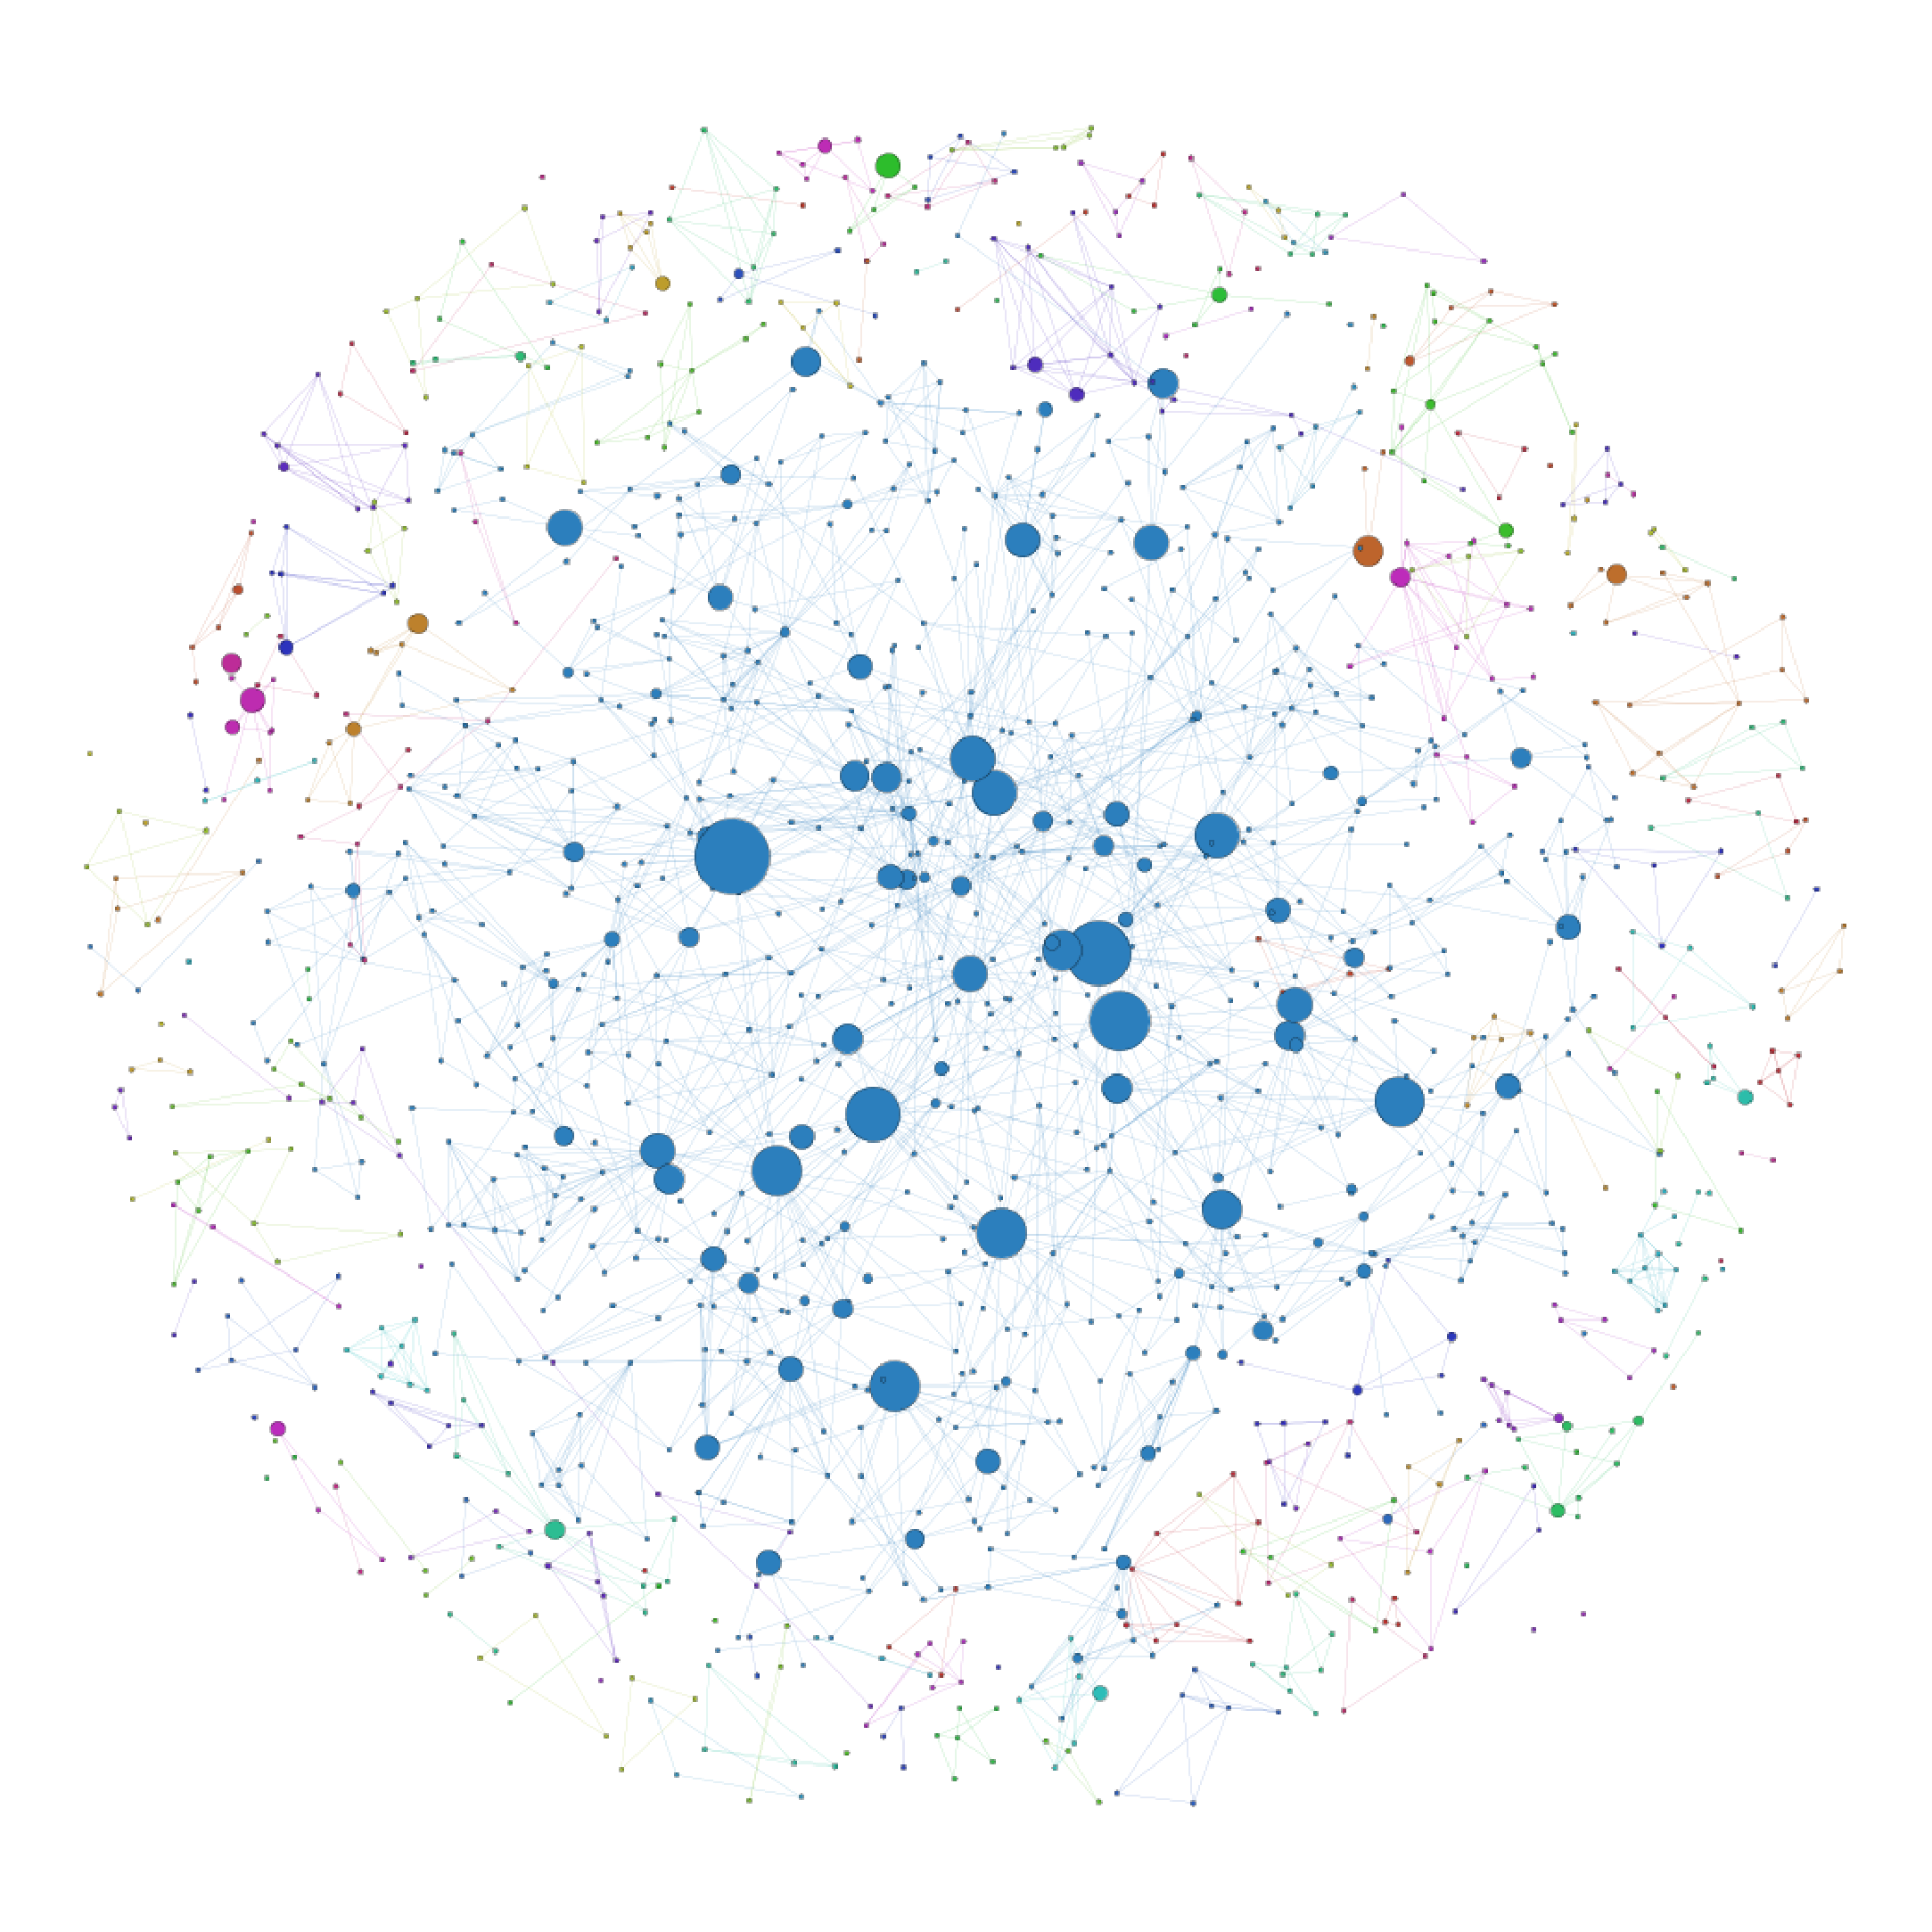
\includegraphics[scale=.21]{../graficos/network/ccs.eps}
  }%
  \subfloat[CIKM]{%
    \label{fig:rede_cikm_apendice}
    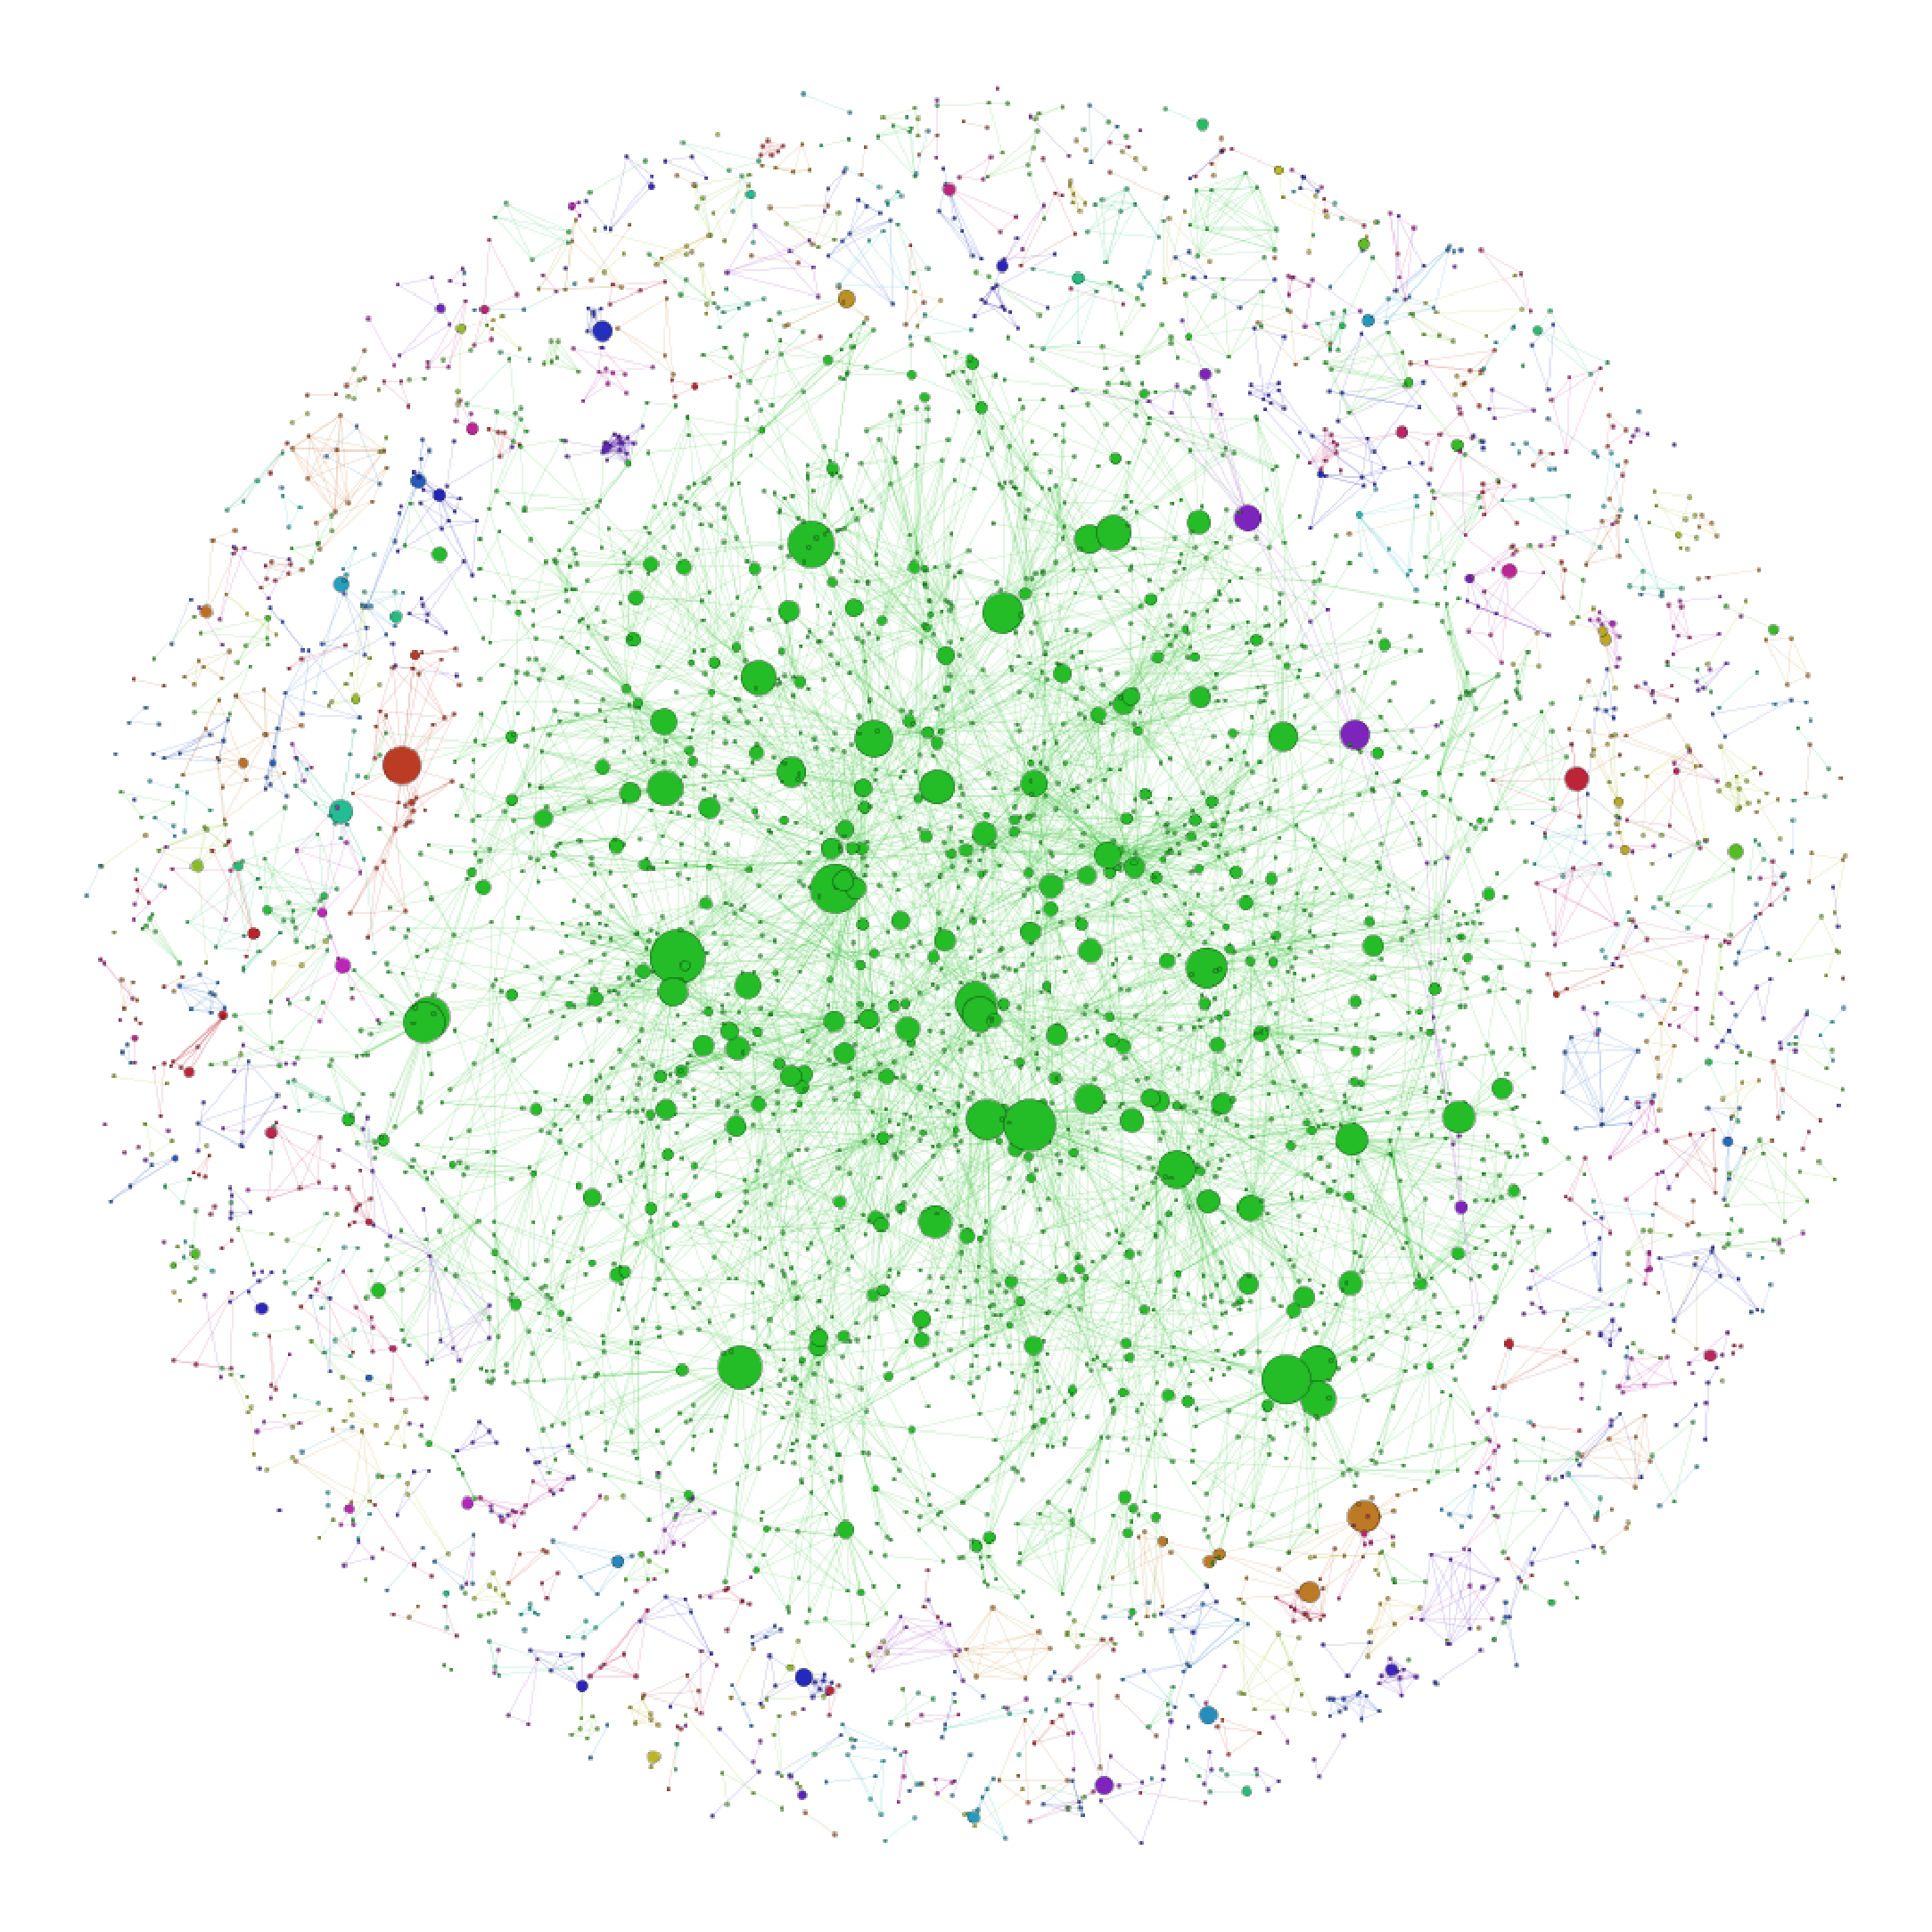
\includegraphics[scale=.21]{../graficos/network/cikm.eps}
  }%
  \phantomcaption
  \end{center}
\end{figure}
\begin{figure}[!htb]
  \begin{center}
  \ContinuedFloat
  \subfloat[DAC]{%
    \label{fig:rede_dac_apendice}
    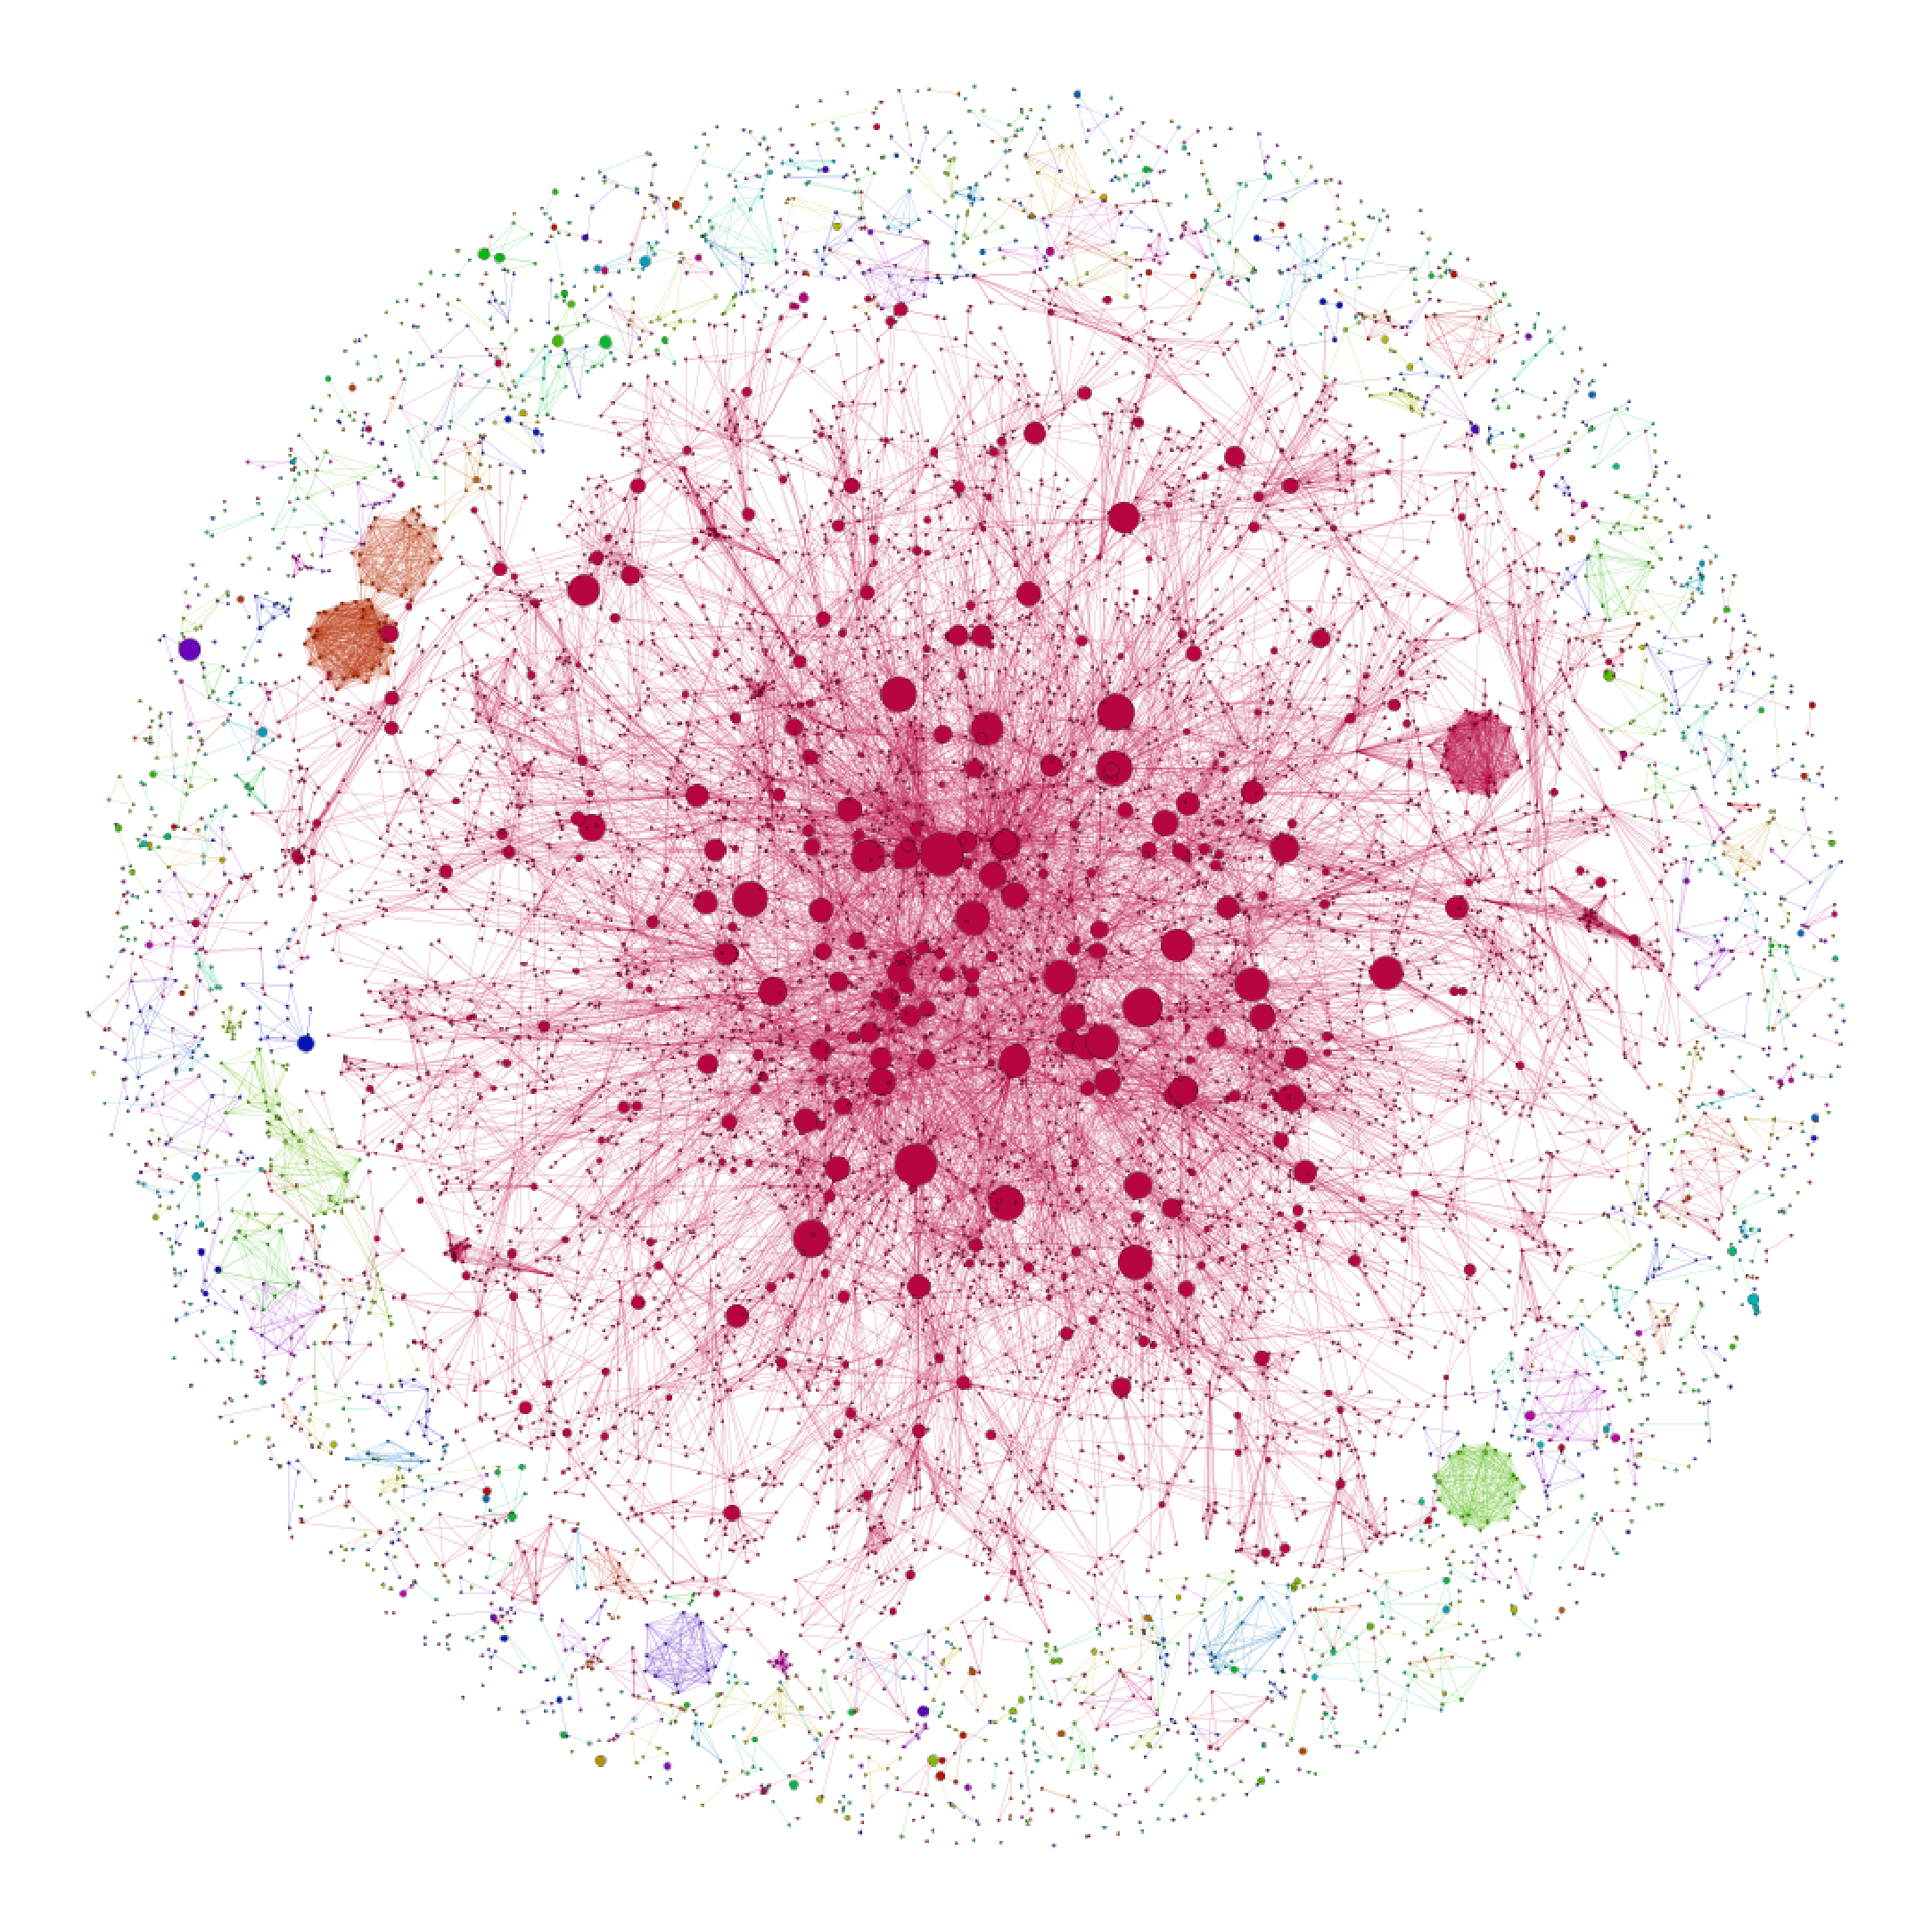
\includegraphics[scale=.21]{../graficos/network/dac.eps}
  }%
  \subfloat[HSCC]{%
    \label{fig:rede_hscc_apendice}
    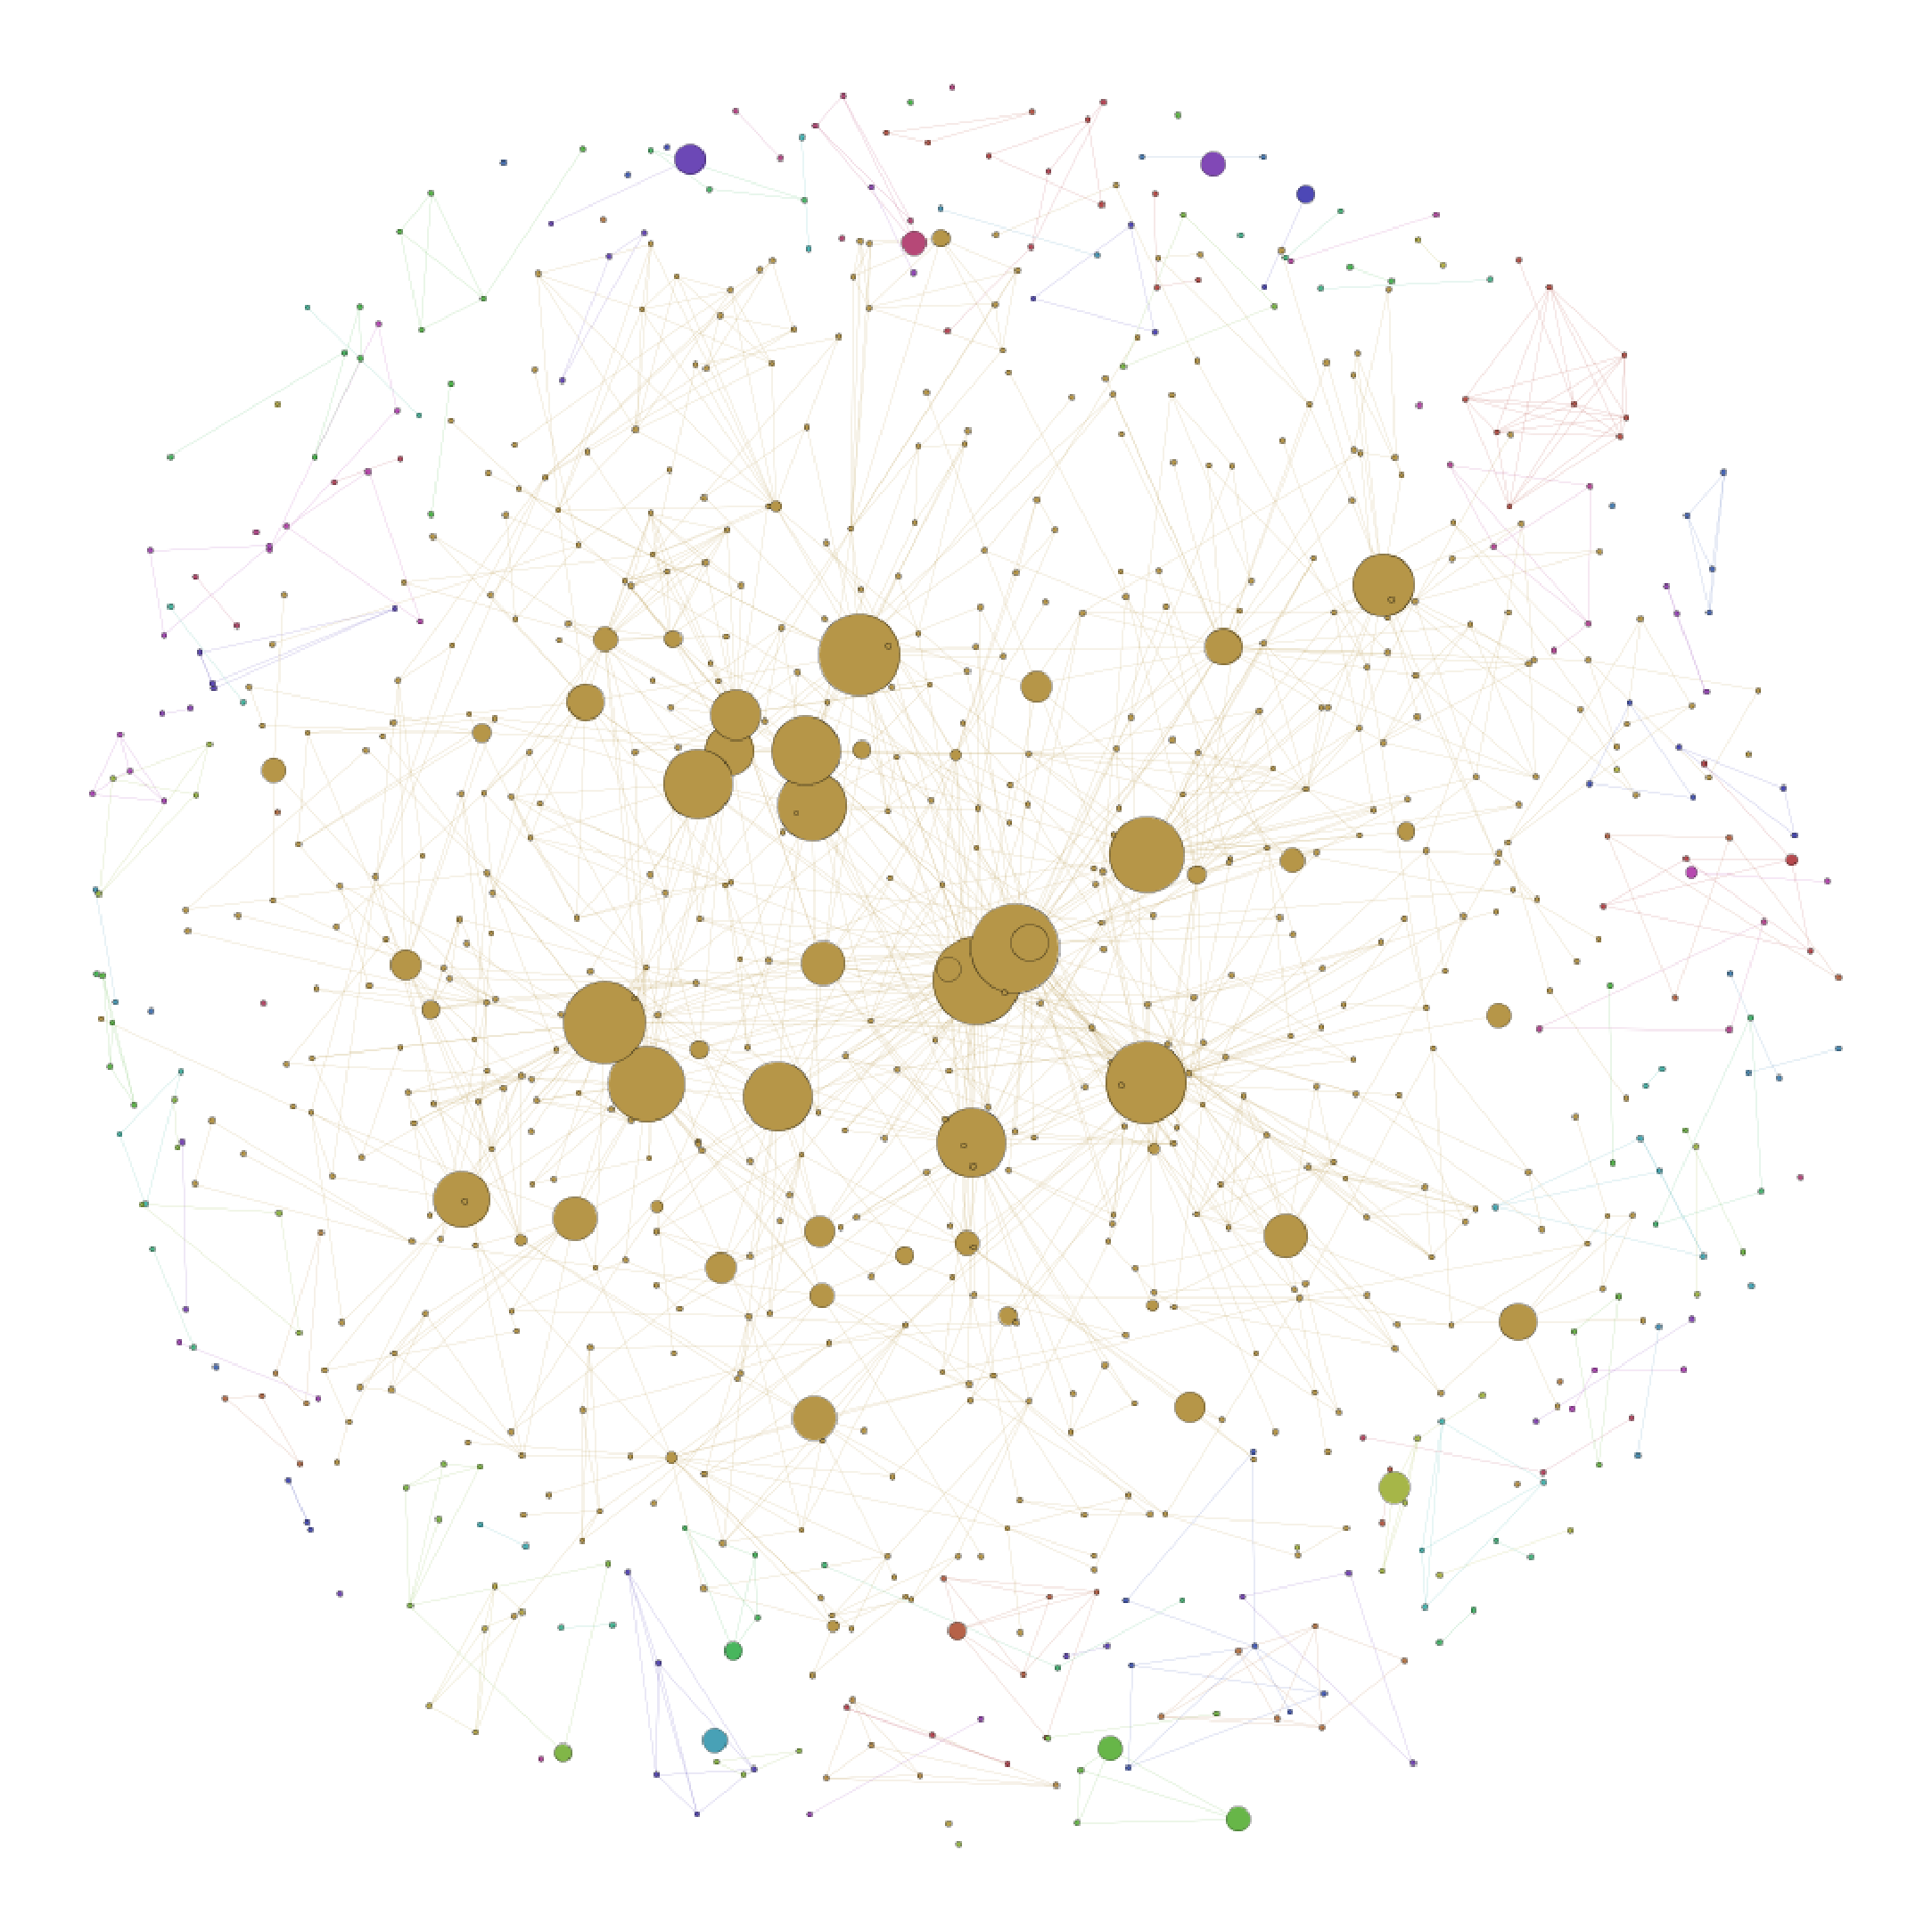
\includegraphics[scale=.21]{../graficos/network/hscc.eps}
  }%
  \\
  \subfloat[ICSE]{%
    \label{fig:rede_icse_apendice}
    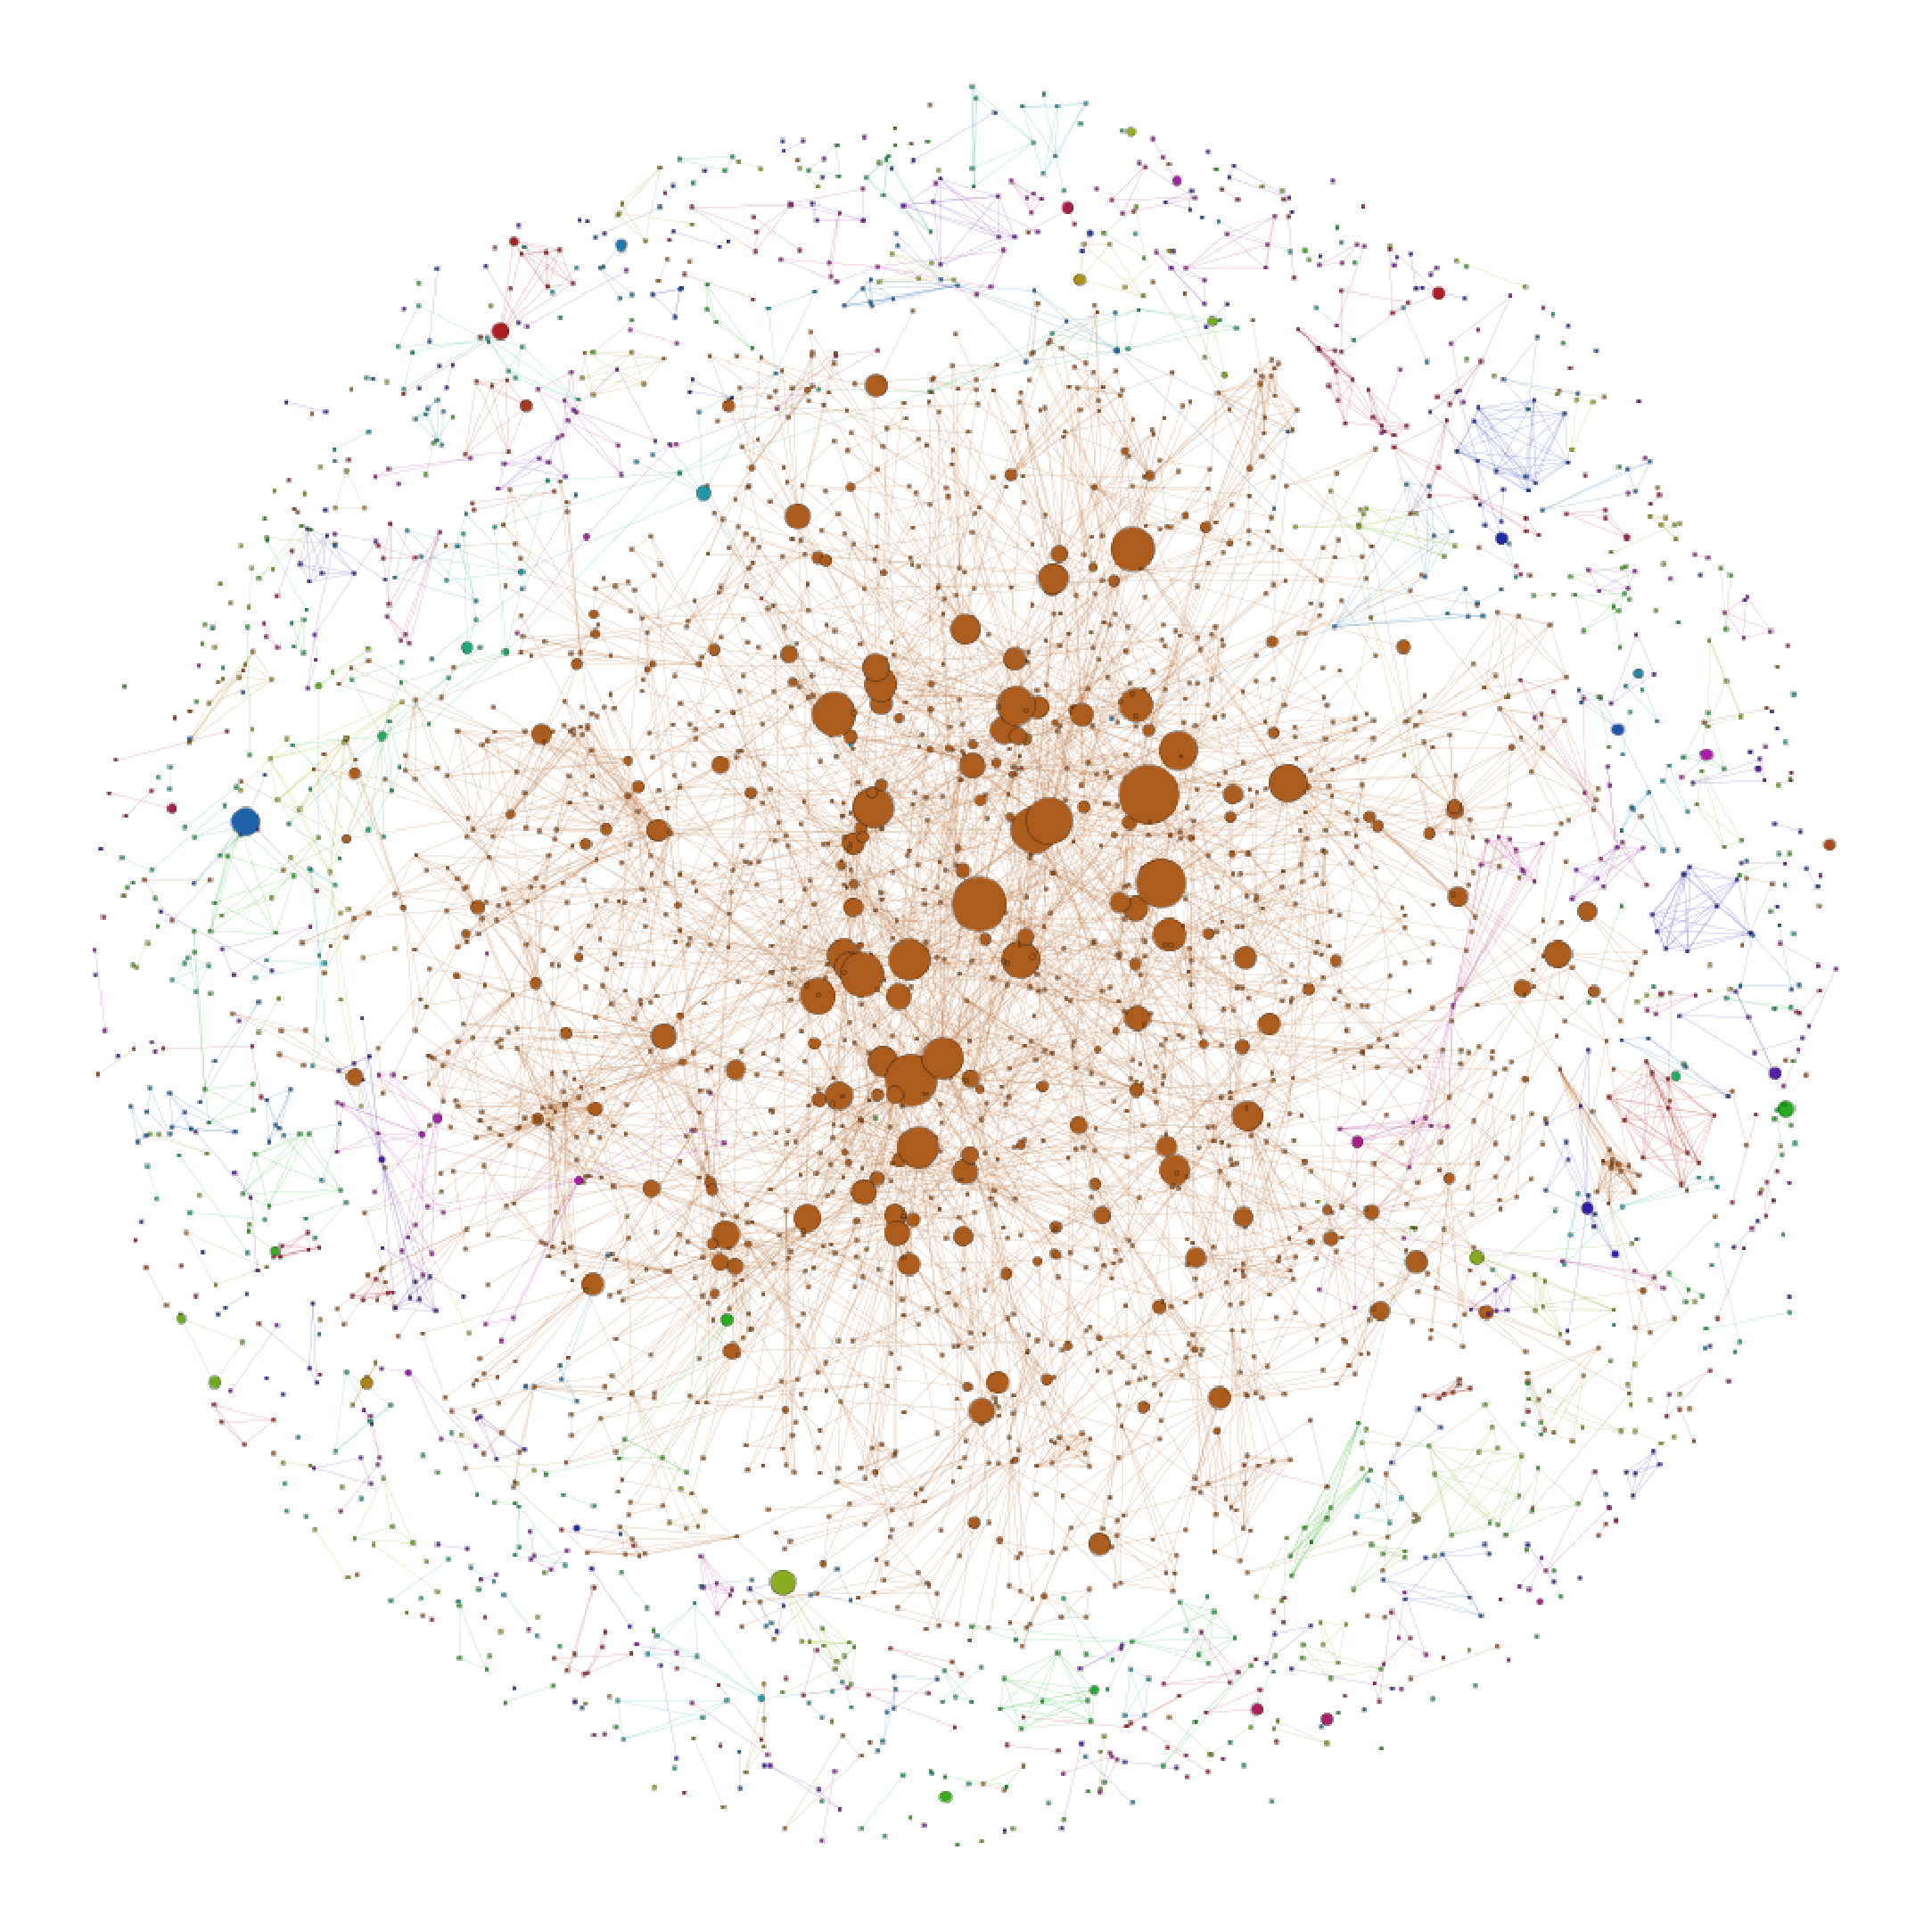
\includegraphics[scale=.21]{../graficos/network/icse.eps}
  }%
  \subfloat[ISCA]{%
    \label{fig:rede_hscc_apendice}
    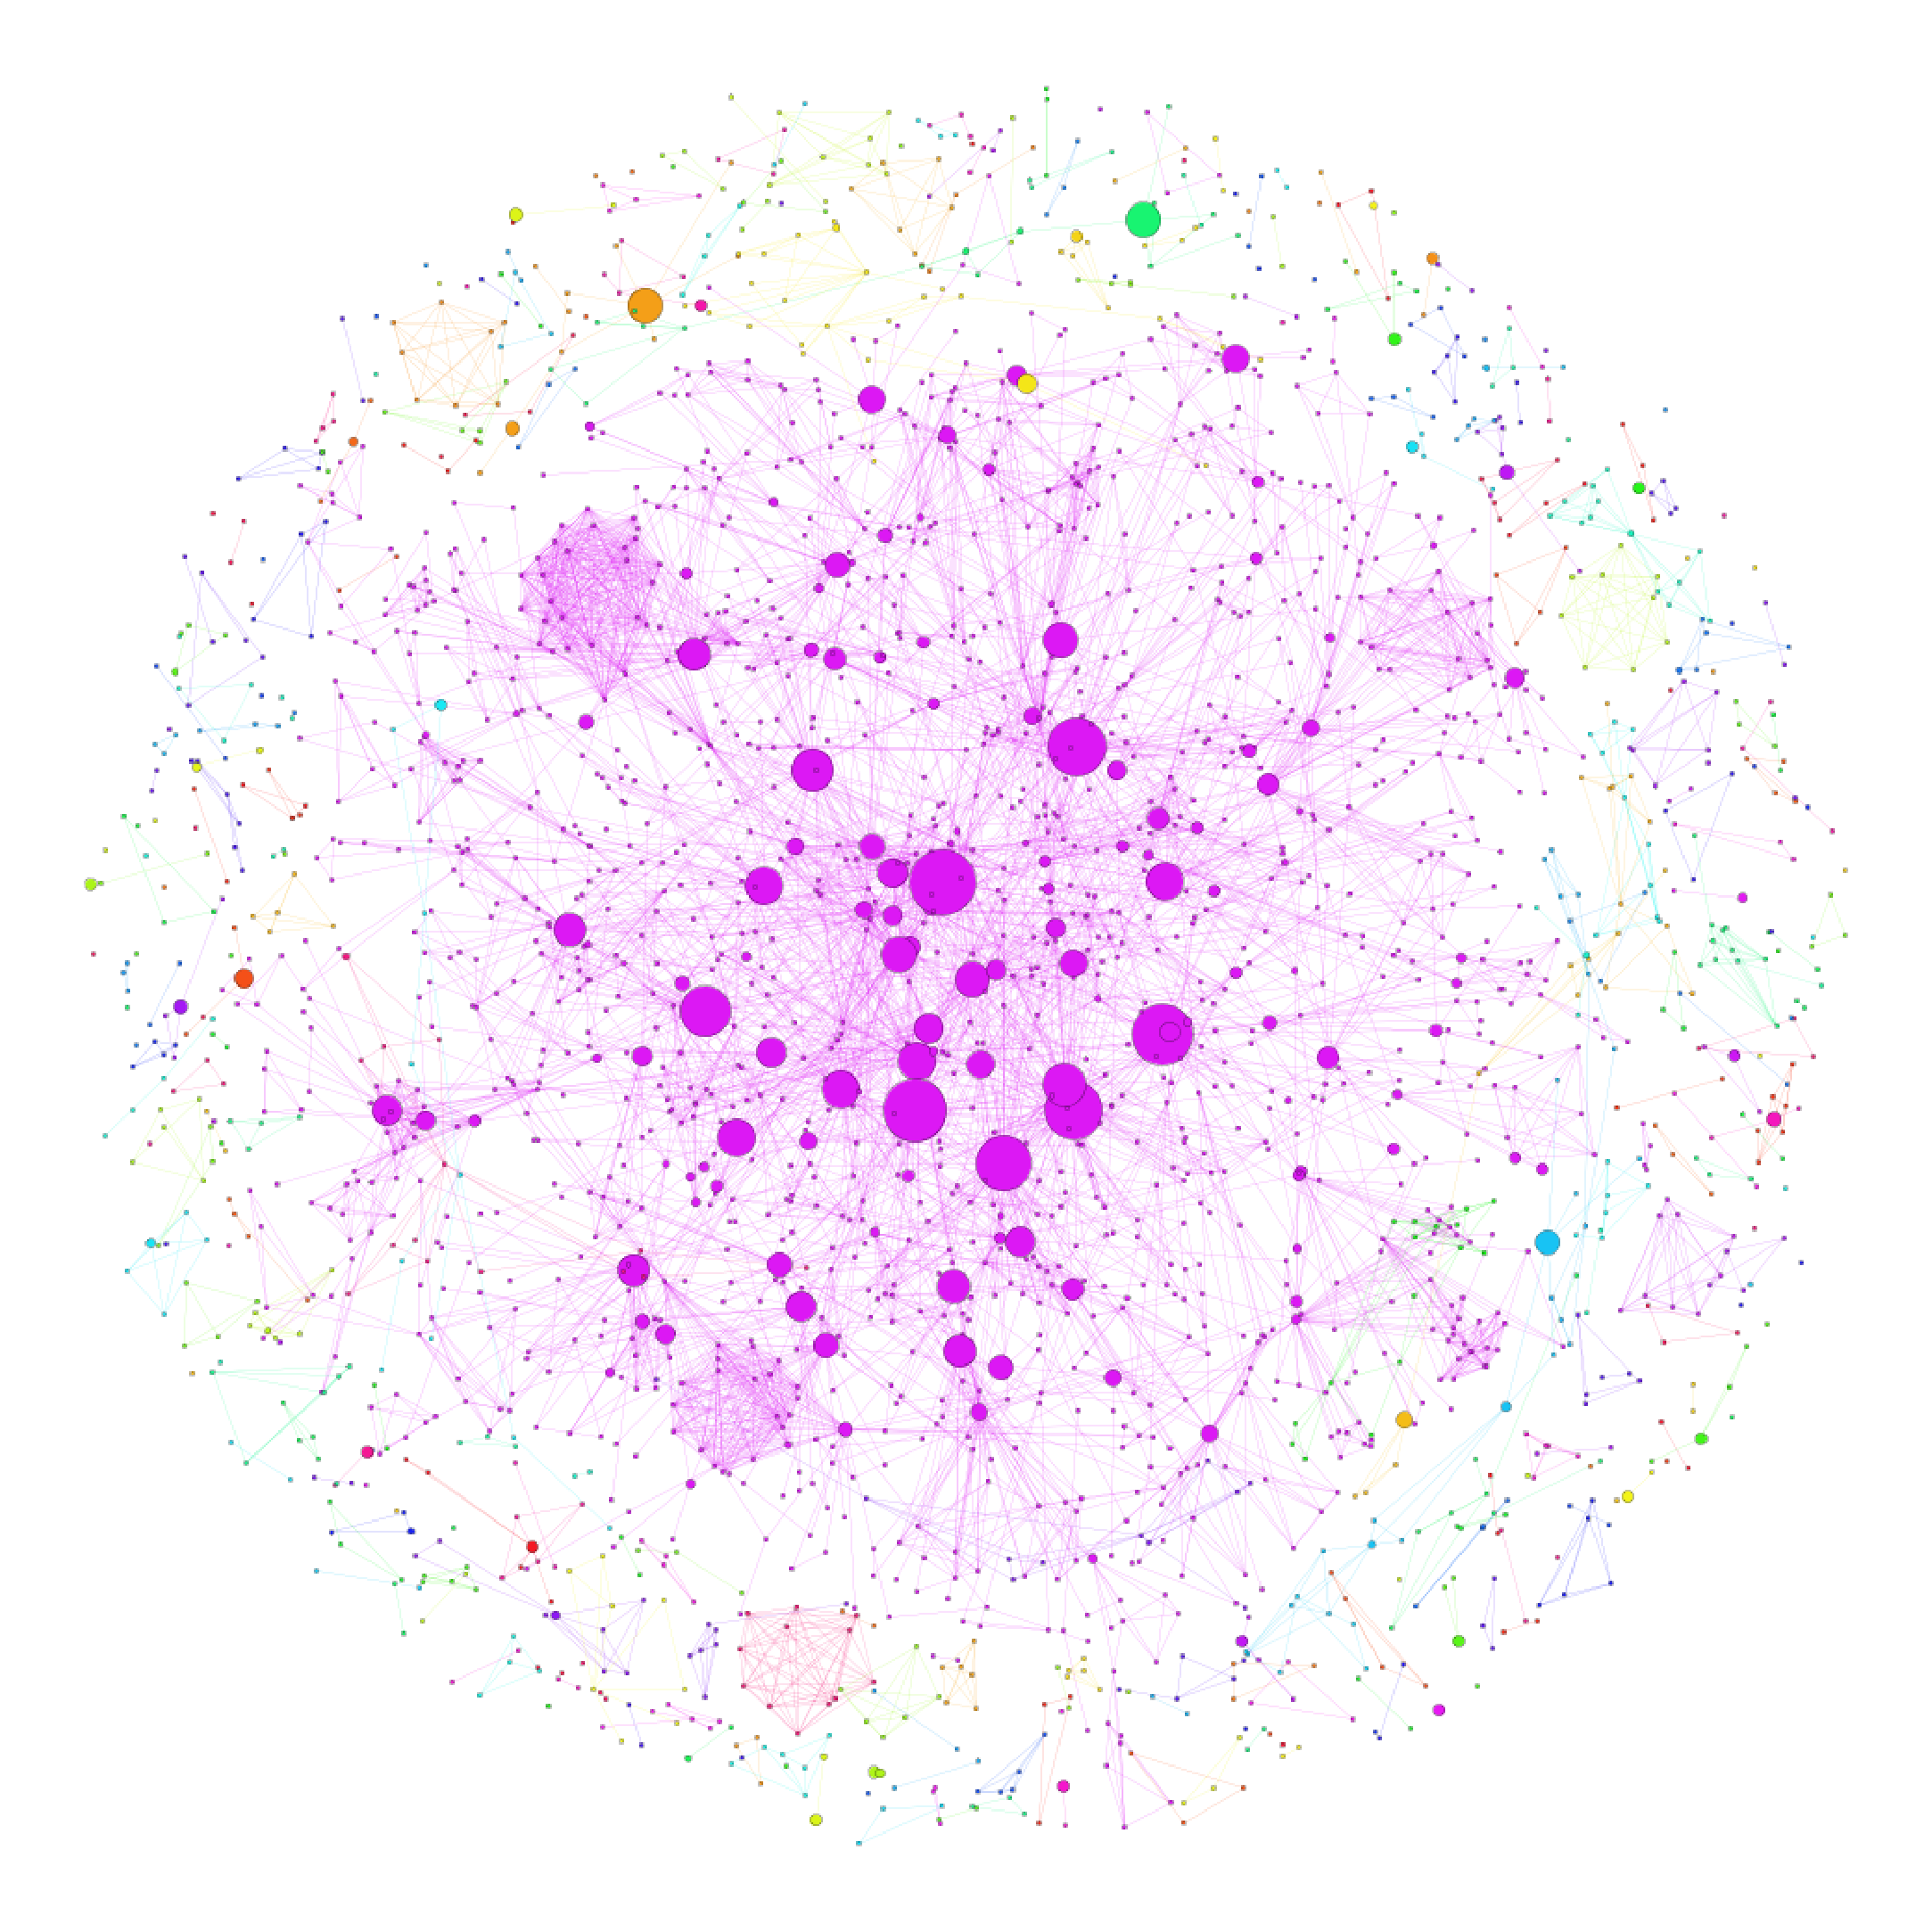
\includegraphics[scale=.21]{../graficos/network/isca.eps}
  }%
  \phantomcaption
  \end{center}
\end{figure}
\begin{figure}[!htb]
  \begin{center}
  \ContinuedFloat
  \subfloat[KDD]{%
    \label{fig:rede_kdd_apendice}
    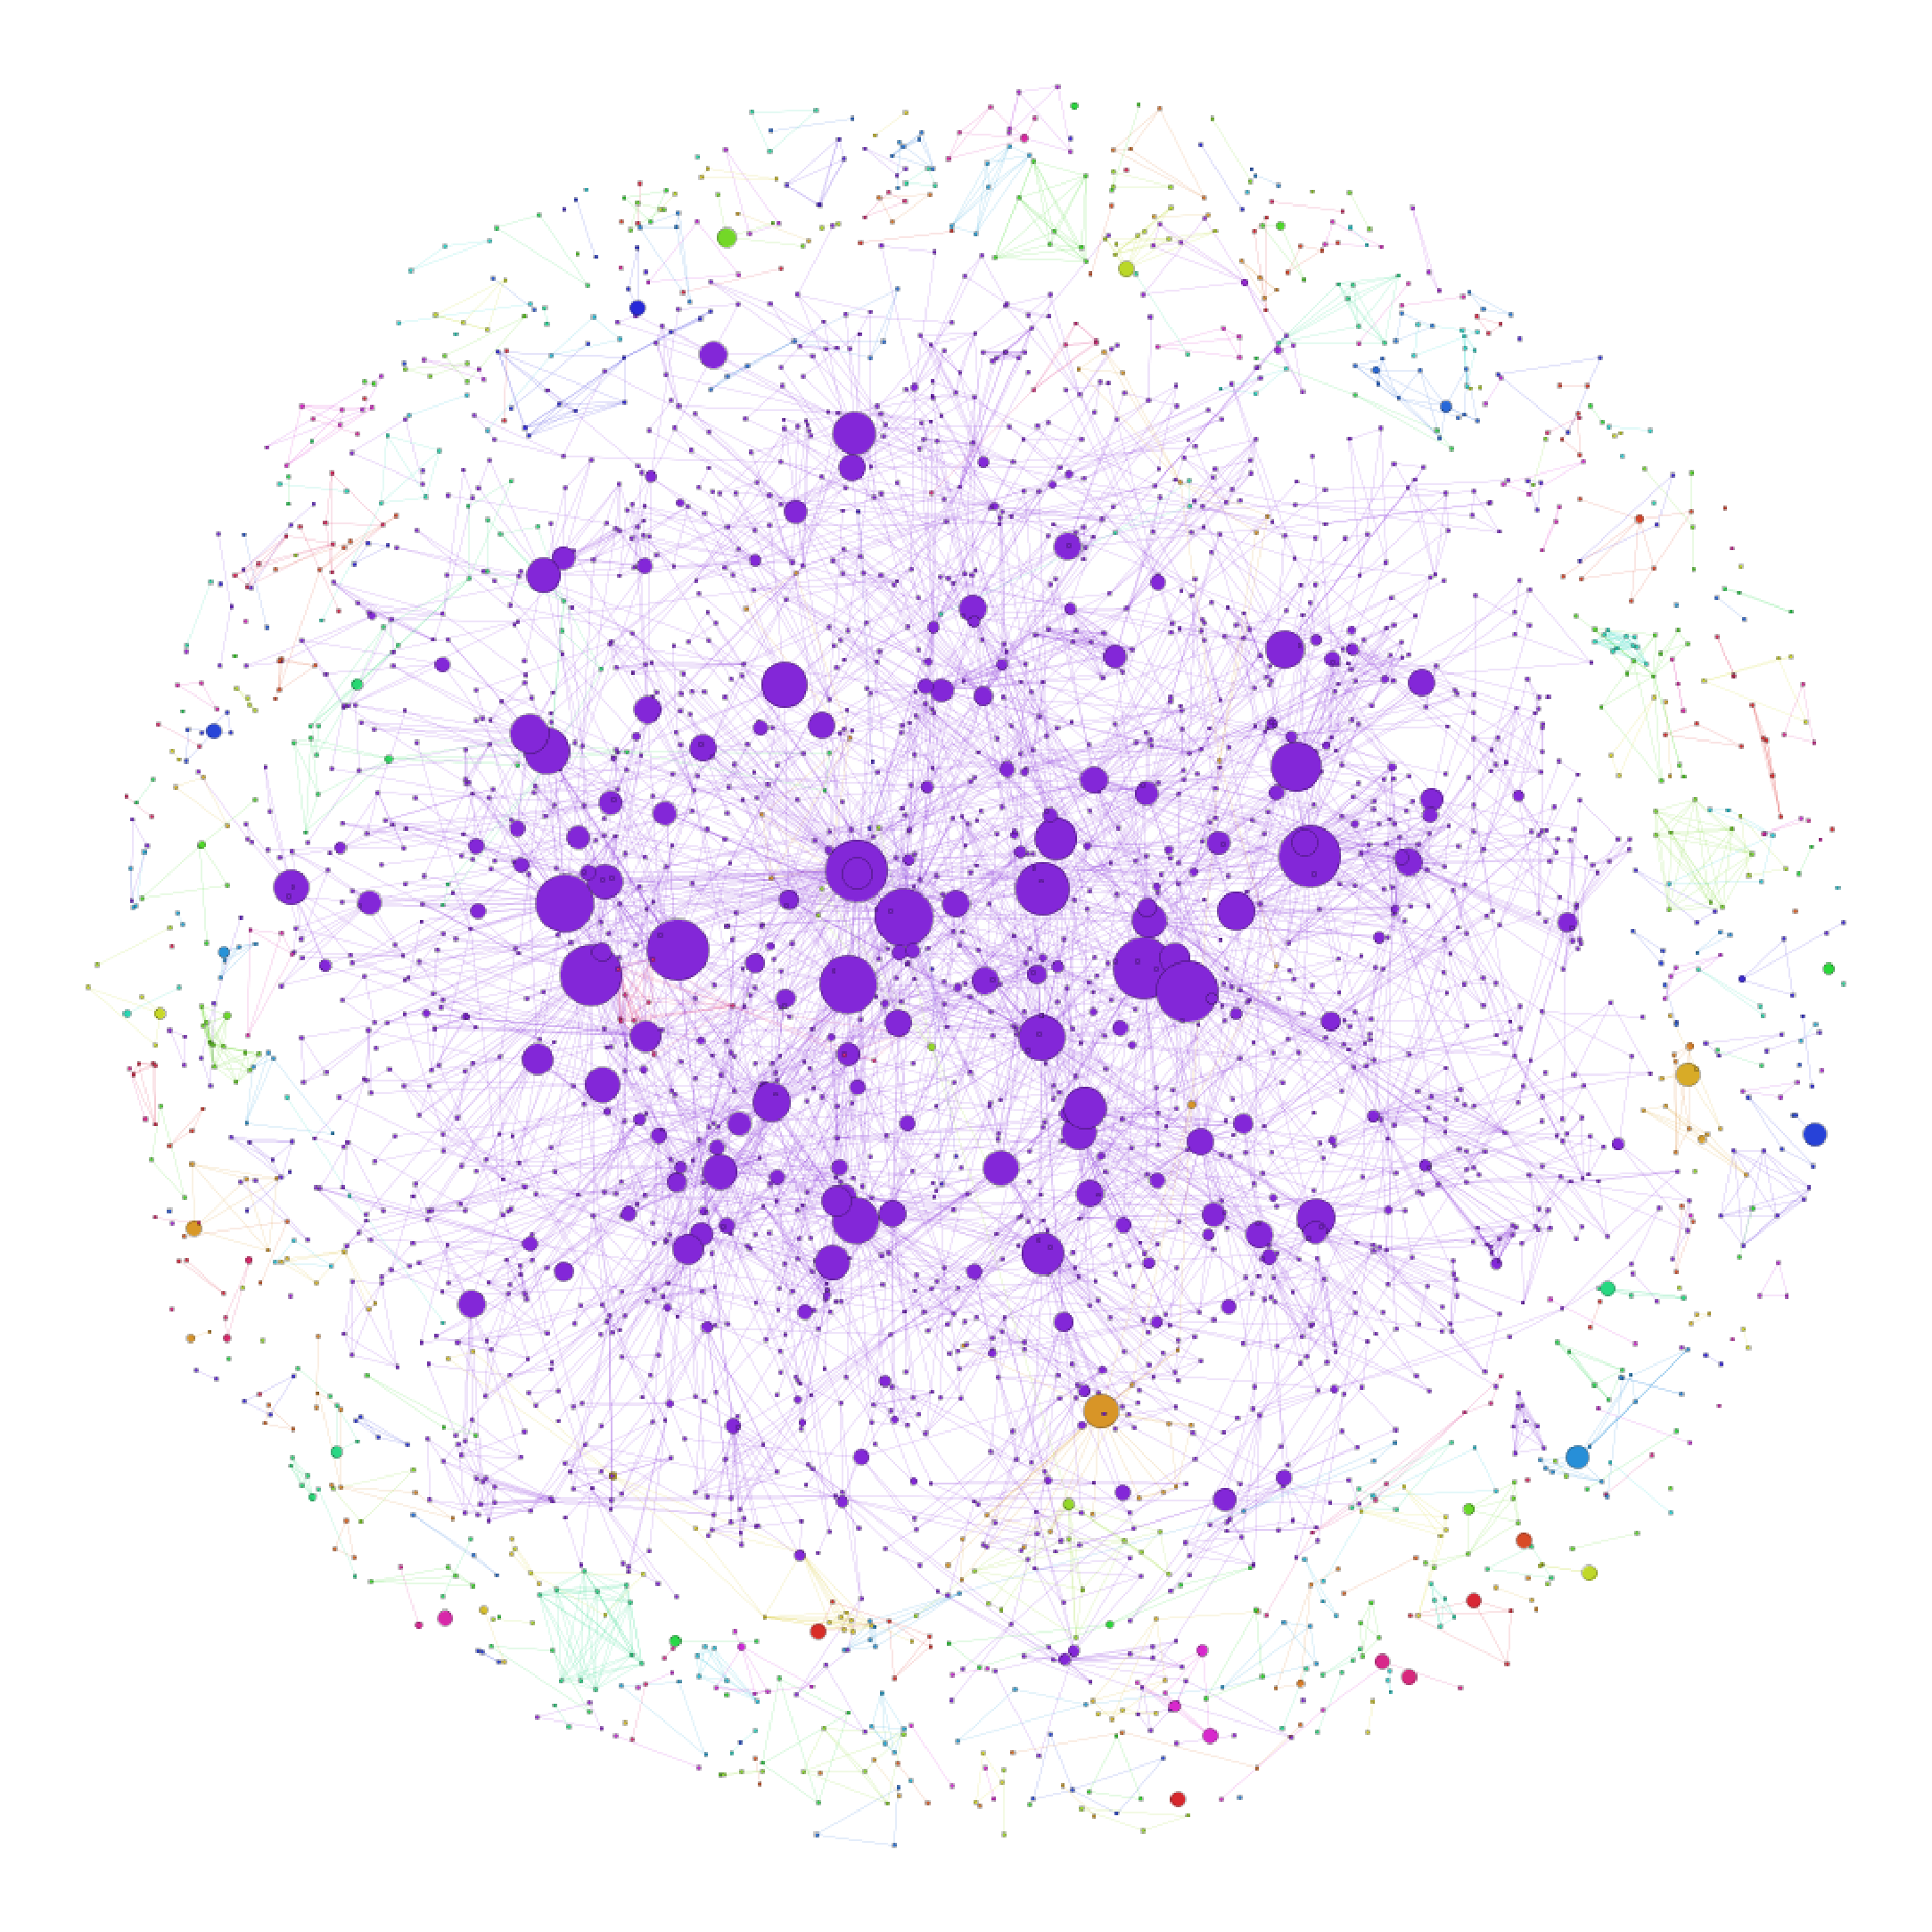
\includegraphics[scale=.21]{../graficos/network/kdd.eps}
  }%
  \subfloat[MICRO]{%
    \label{fig:rede_micro_apendice}
    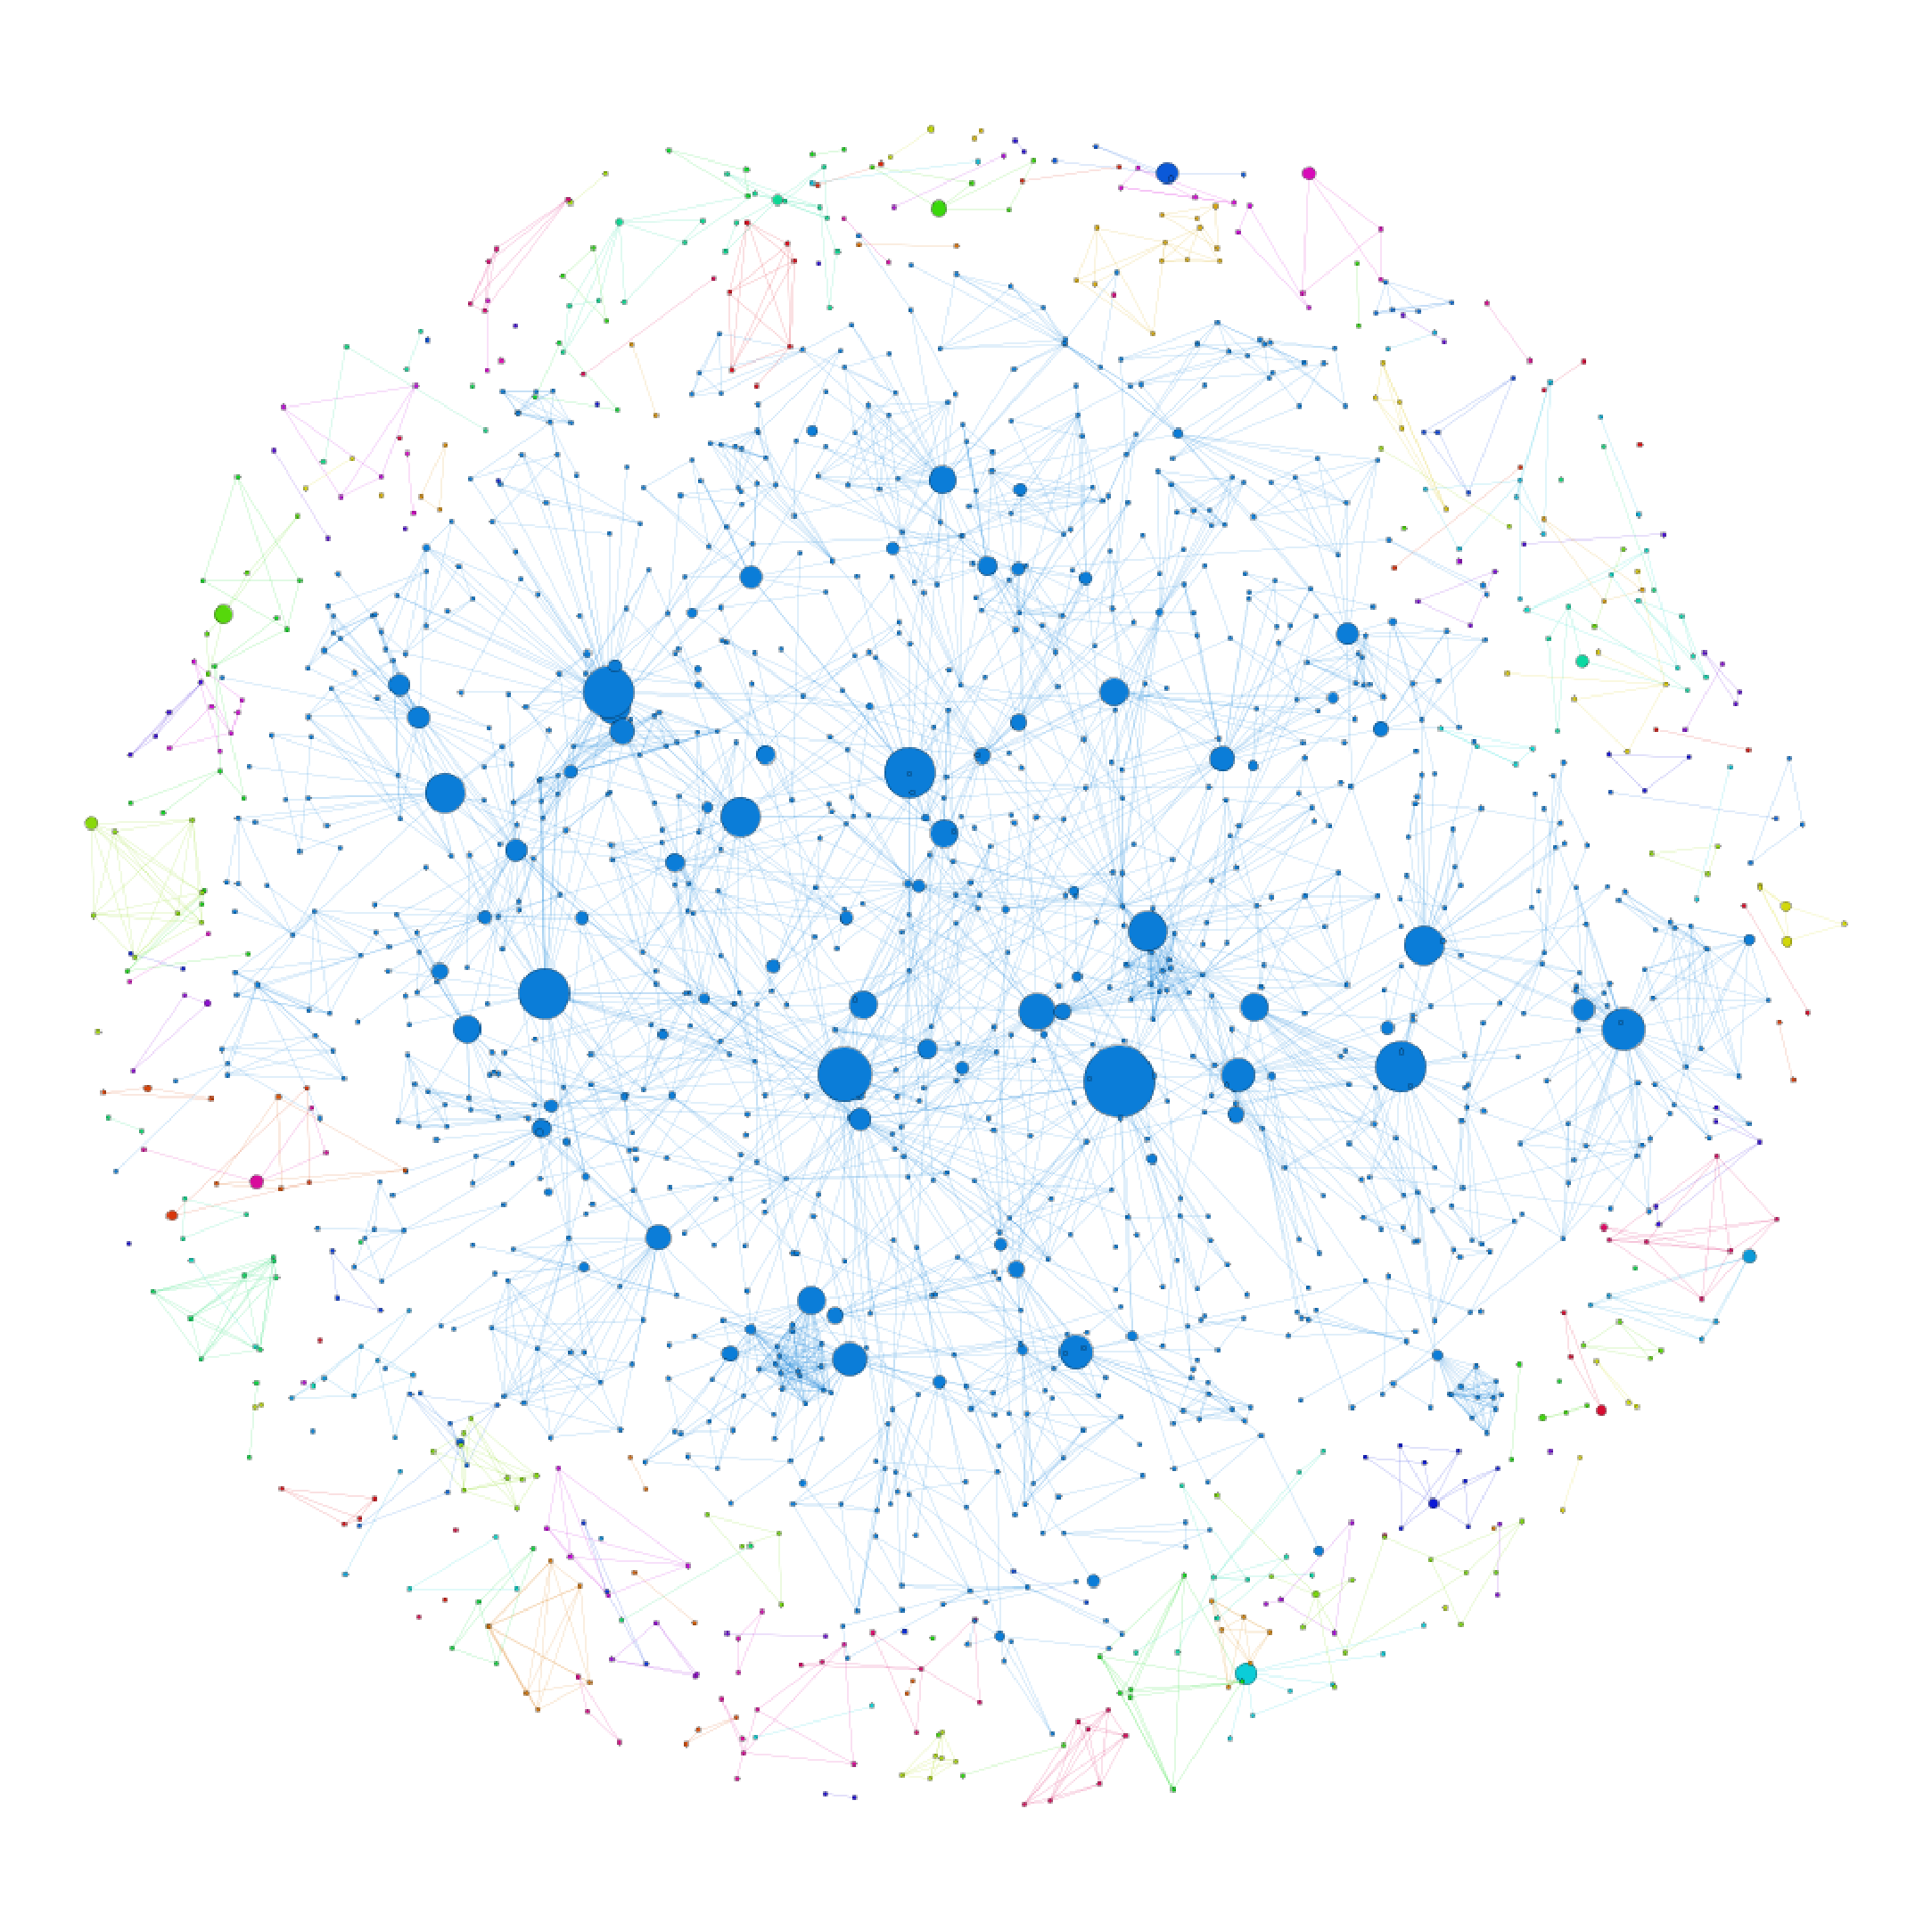
\includegraphics[scale=.21]{../graficos/network/micro.eps}
  }%
  \\
  \subfloat[MM]{%
    \label{fig:rede_mm_apendice}
    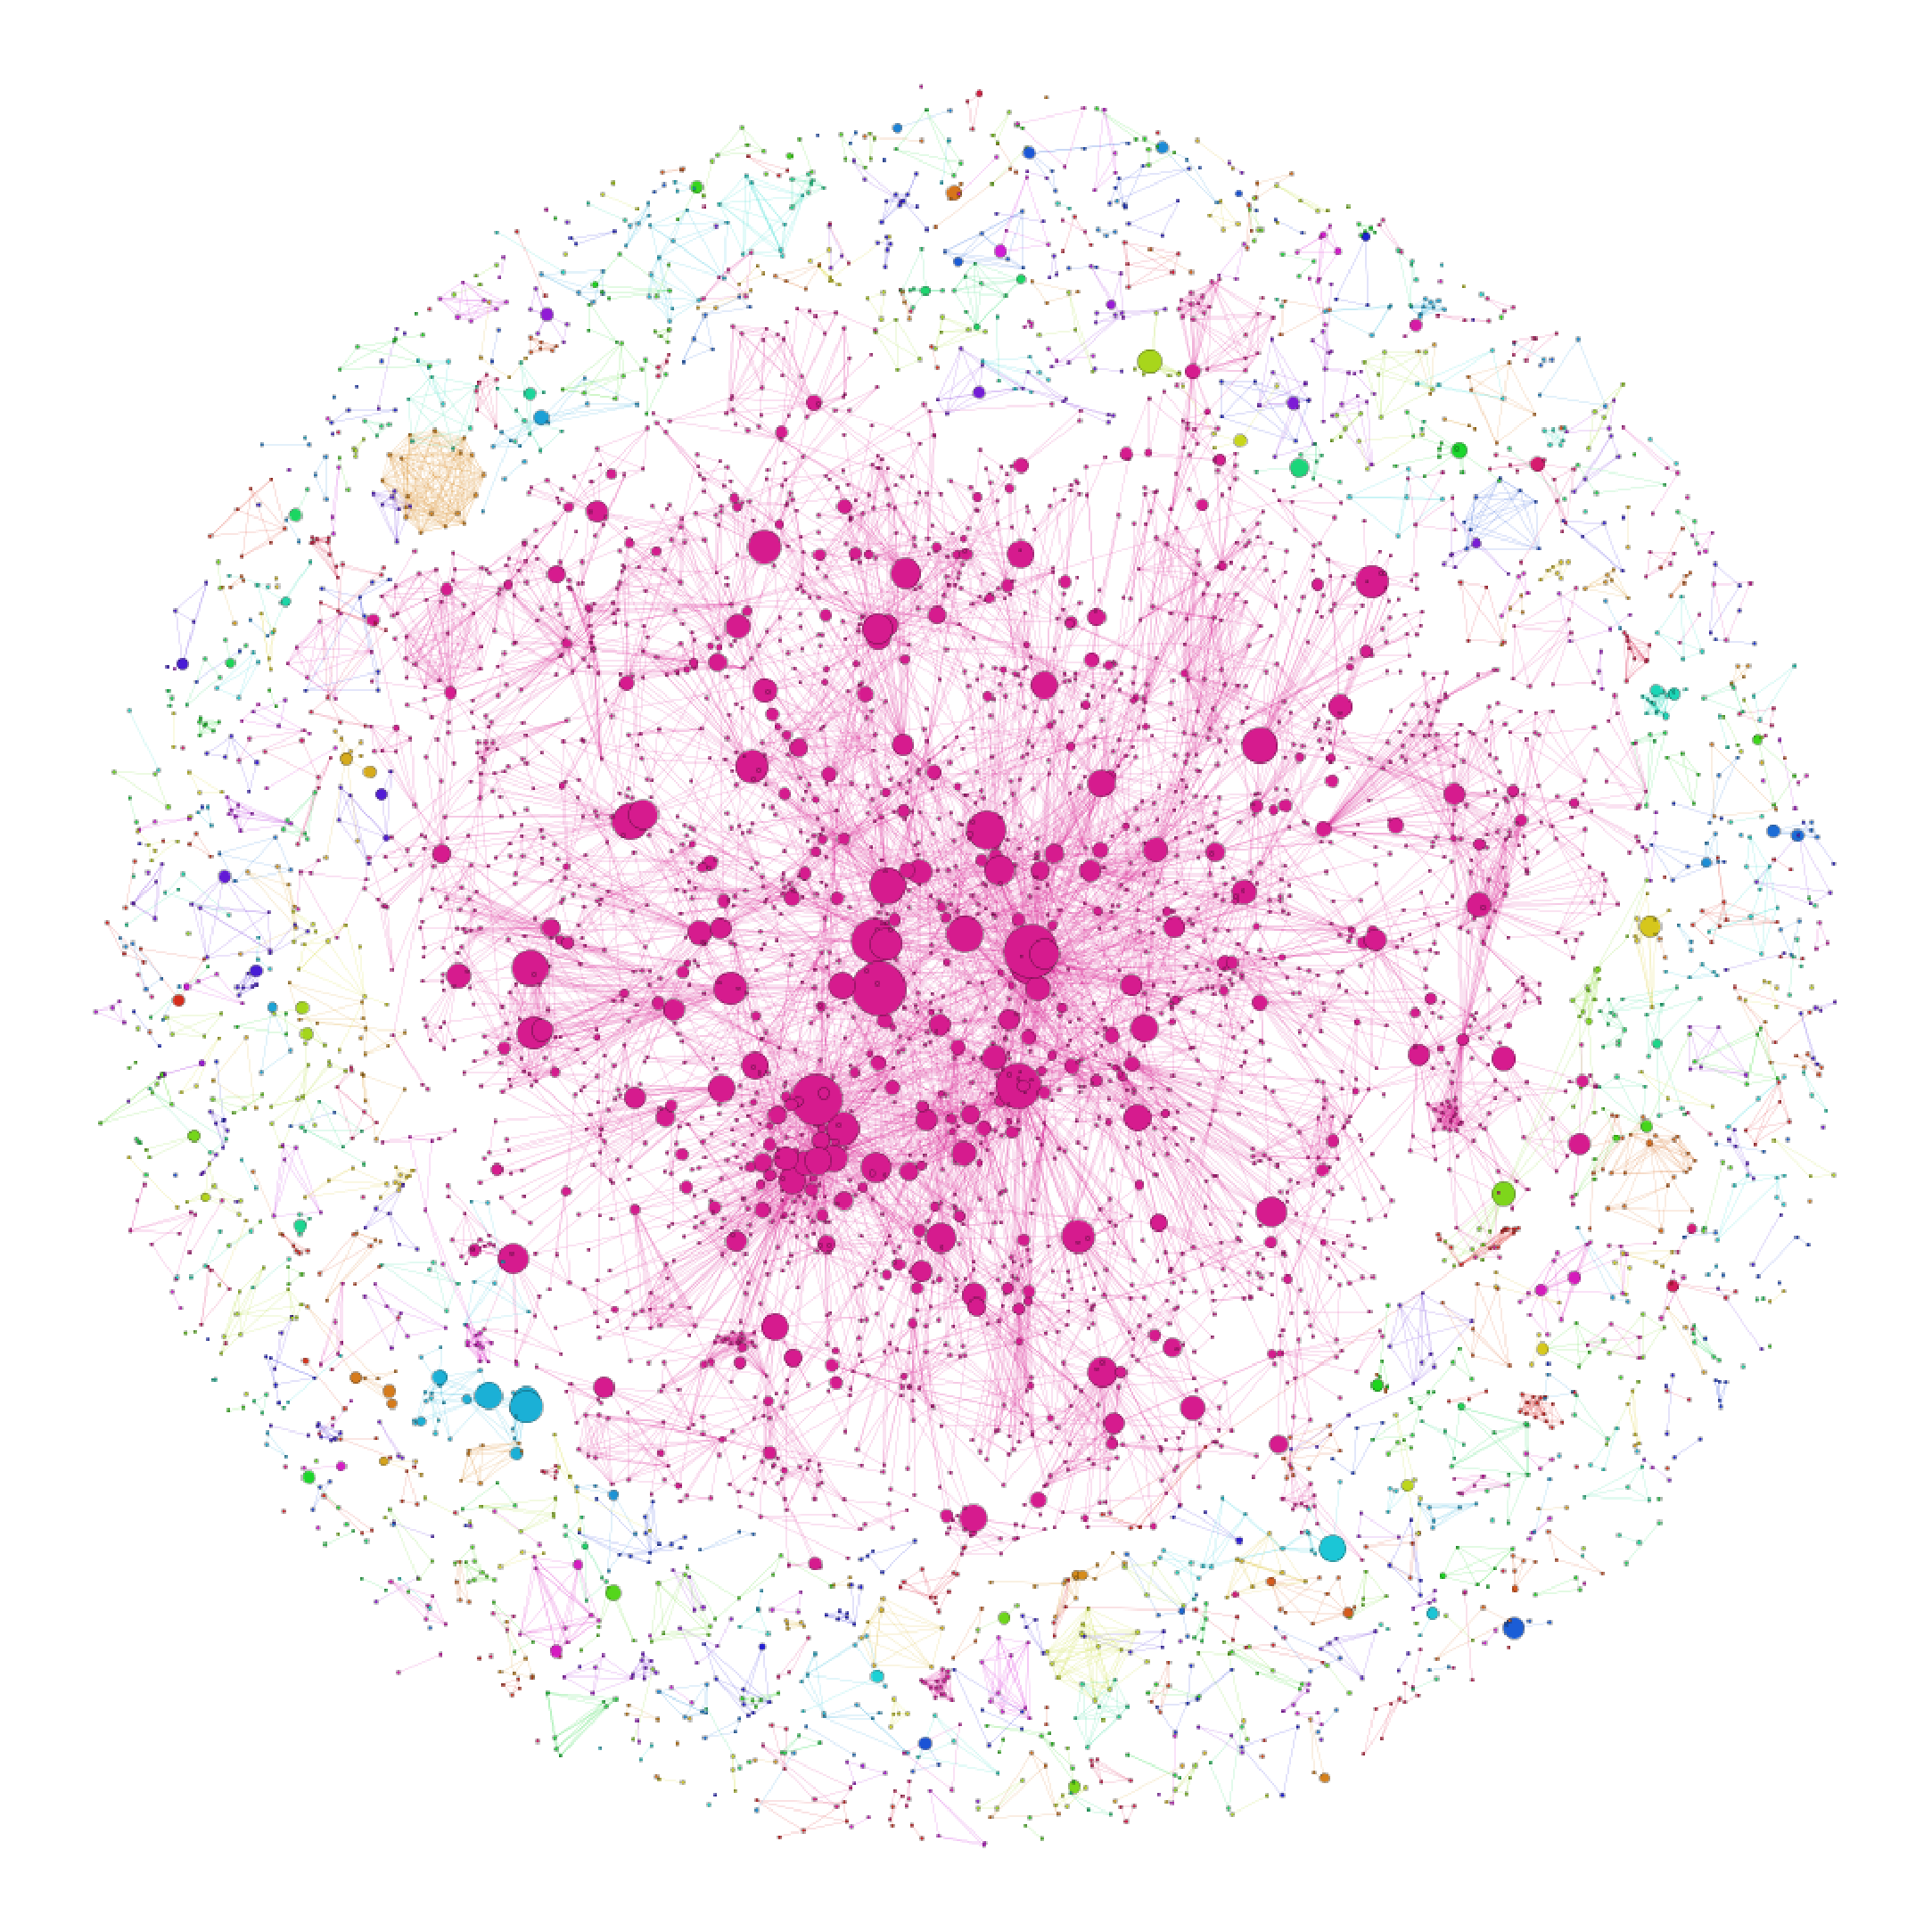
\includegraphics[scale=.21]{../graficos/network/acm_multimedia.eps}
  }%
  \subfloat[MOBICOM]{%
    \label{fig:rede_mobicom_apendice}
    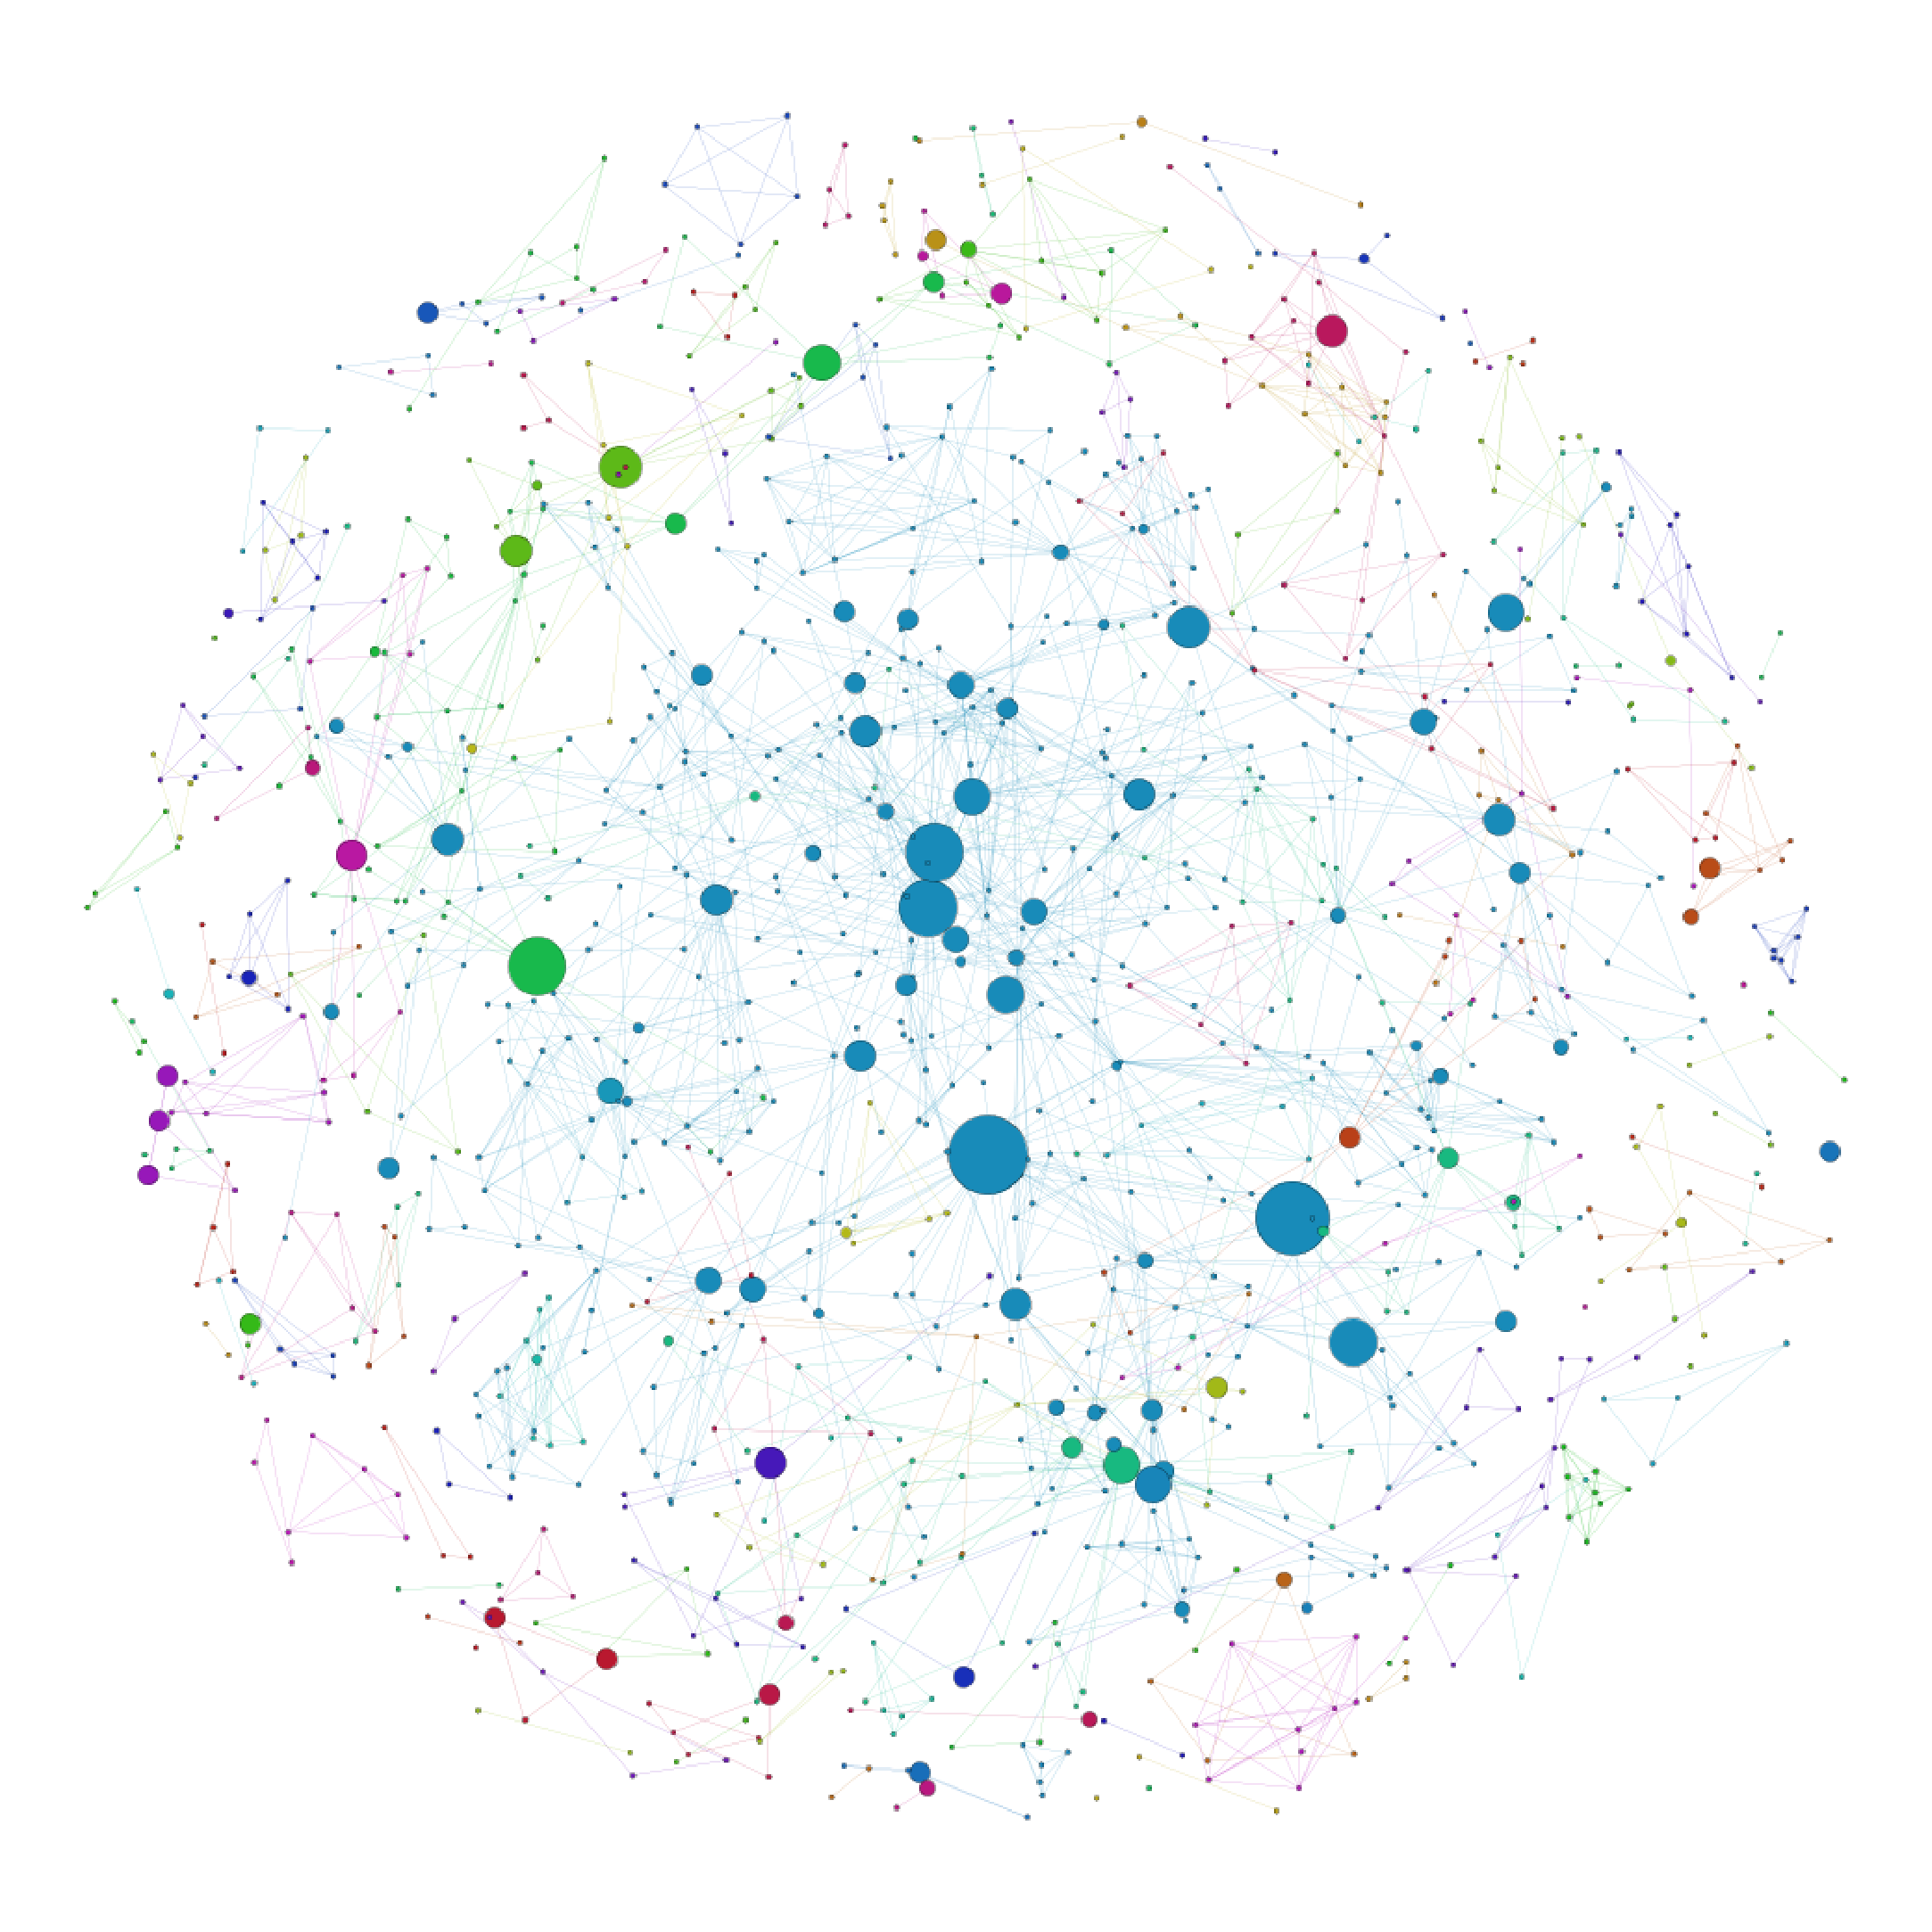
\includegraphics[scale=.21]{../graficos/network/mobicom.eps}
  }%
  \phantomcaption
  \end{center}
\end{figure}
\begin{figure}[!htb]
  \begin{center}
  \ContinuedFloat
  \subfloat[PODC]{%
    \label{fig:rede_podc_apendice}
    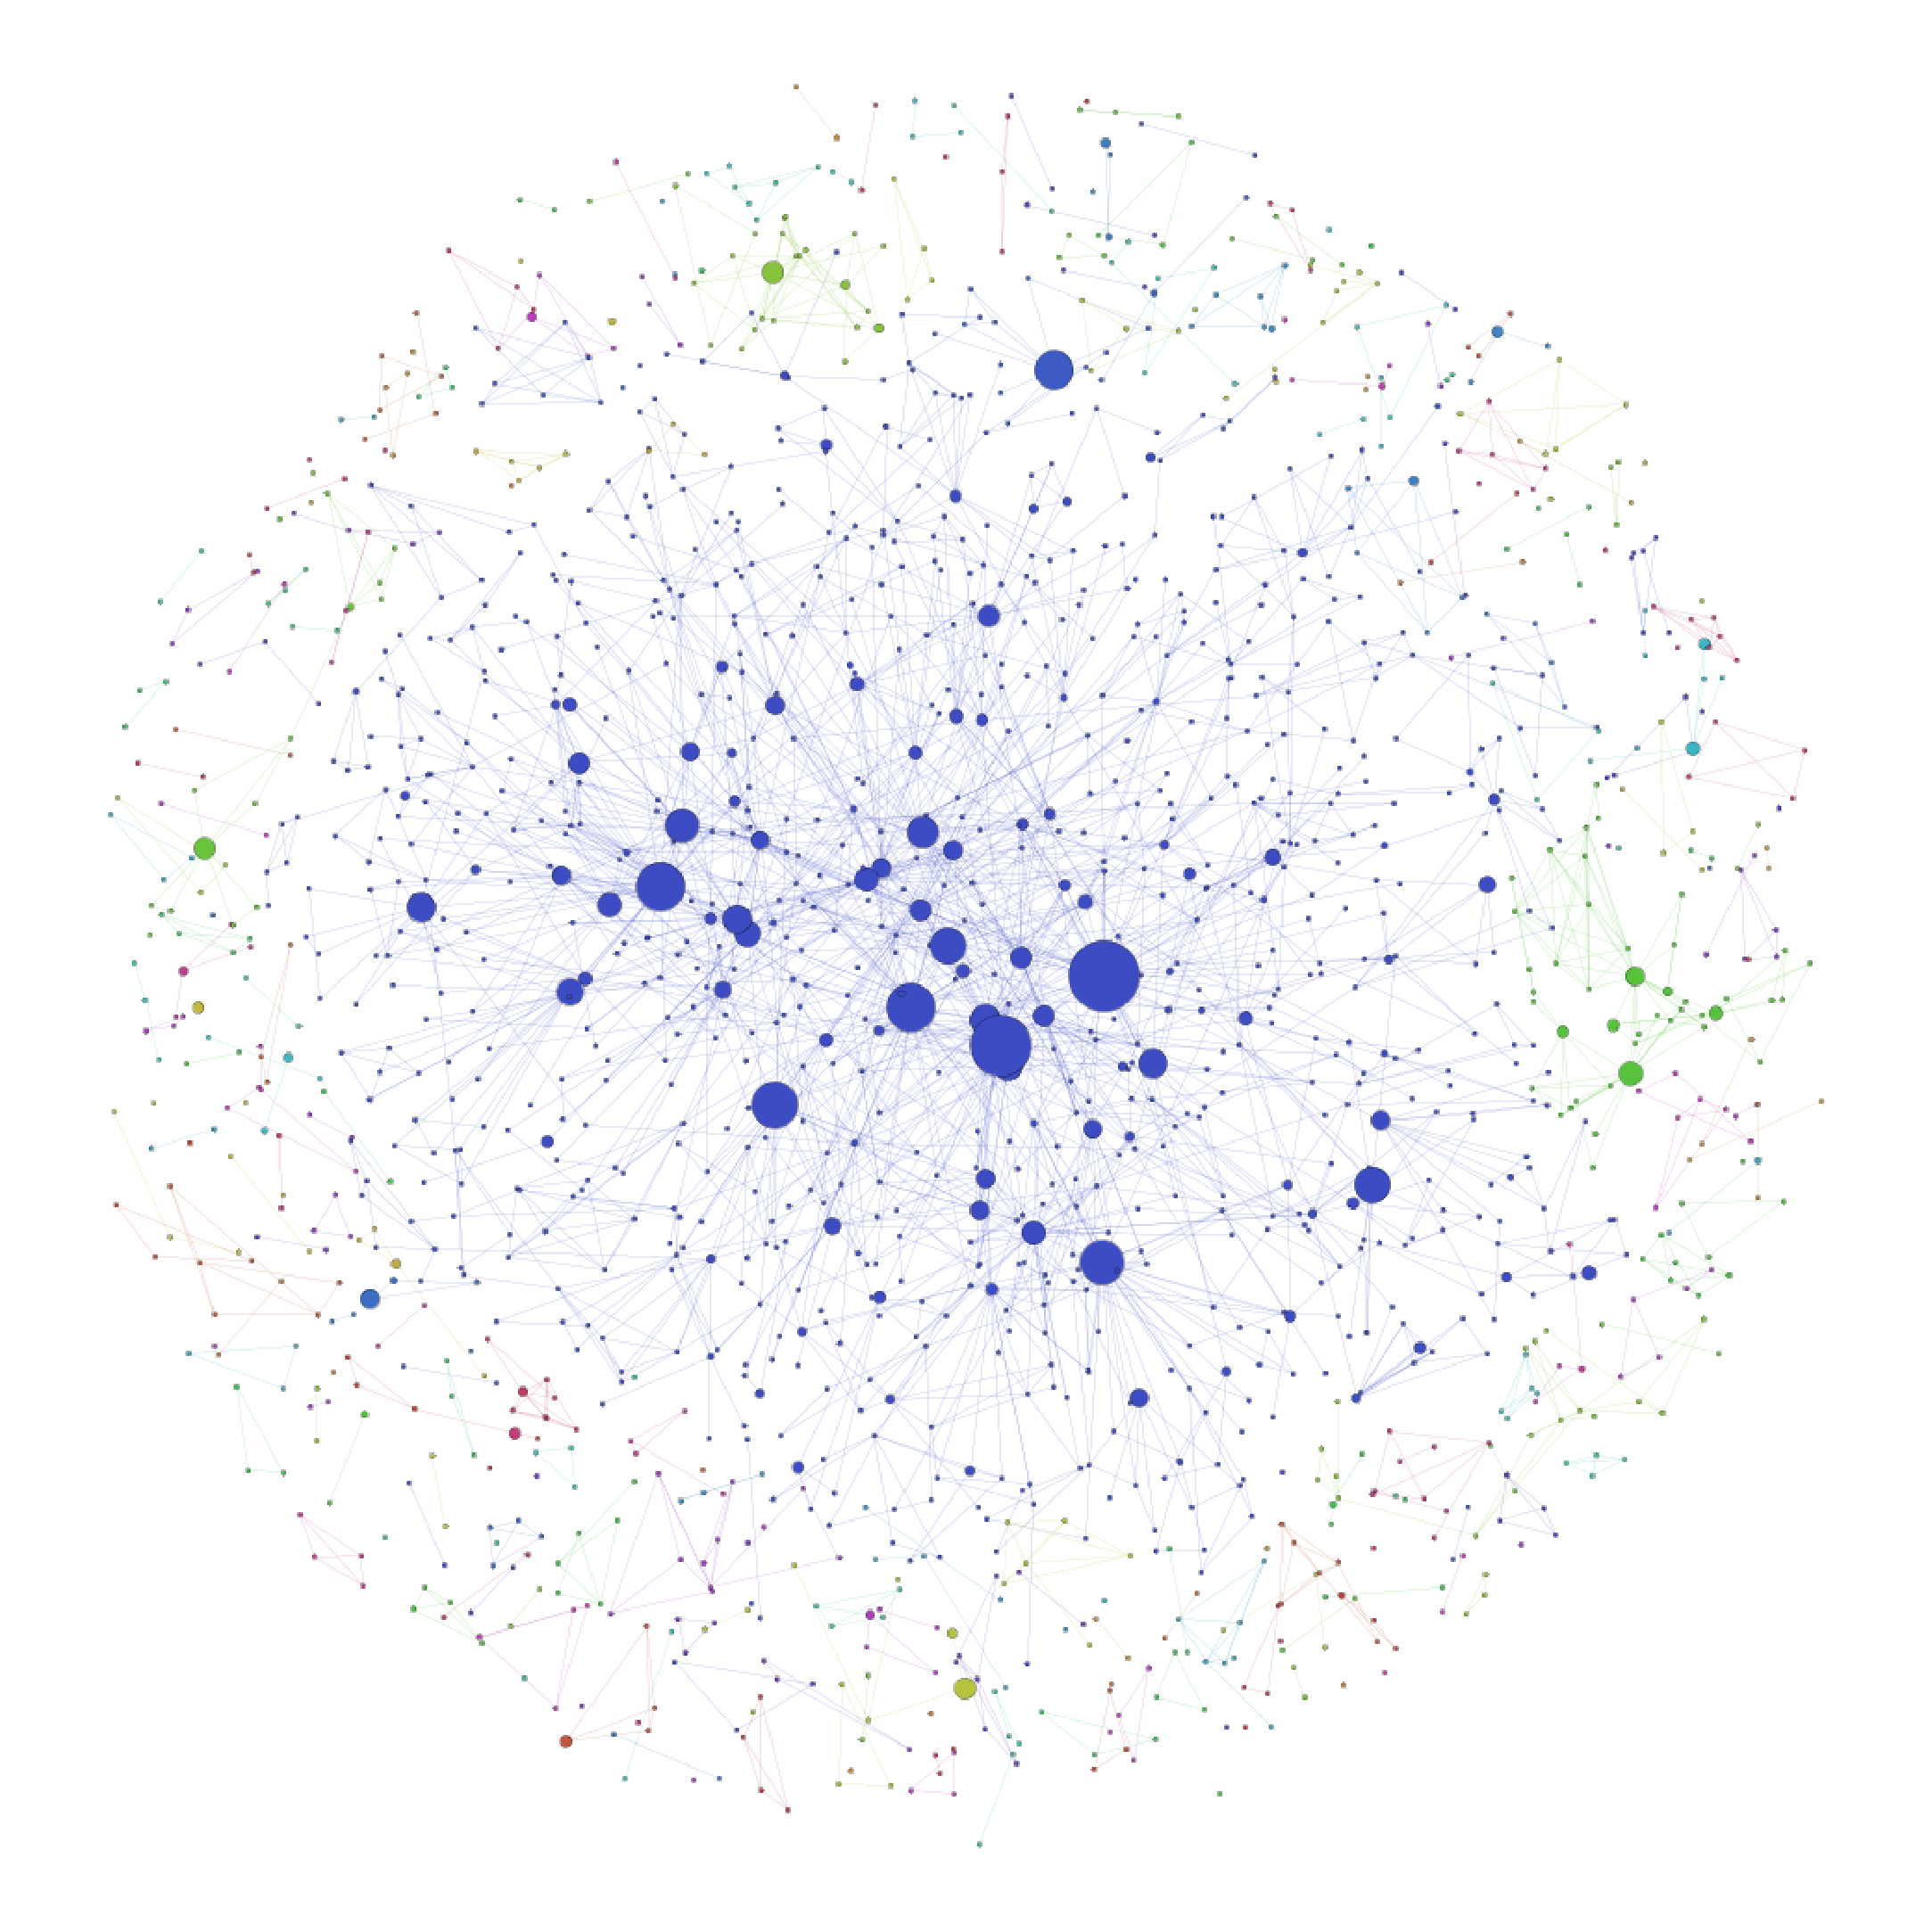
\includegraphics[scale=.21]{../graficos/network/podc.eps}
  }%
  \subfloat[POPL]{%
    \label{fig:rede_popl_apendice}
    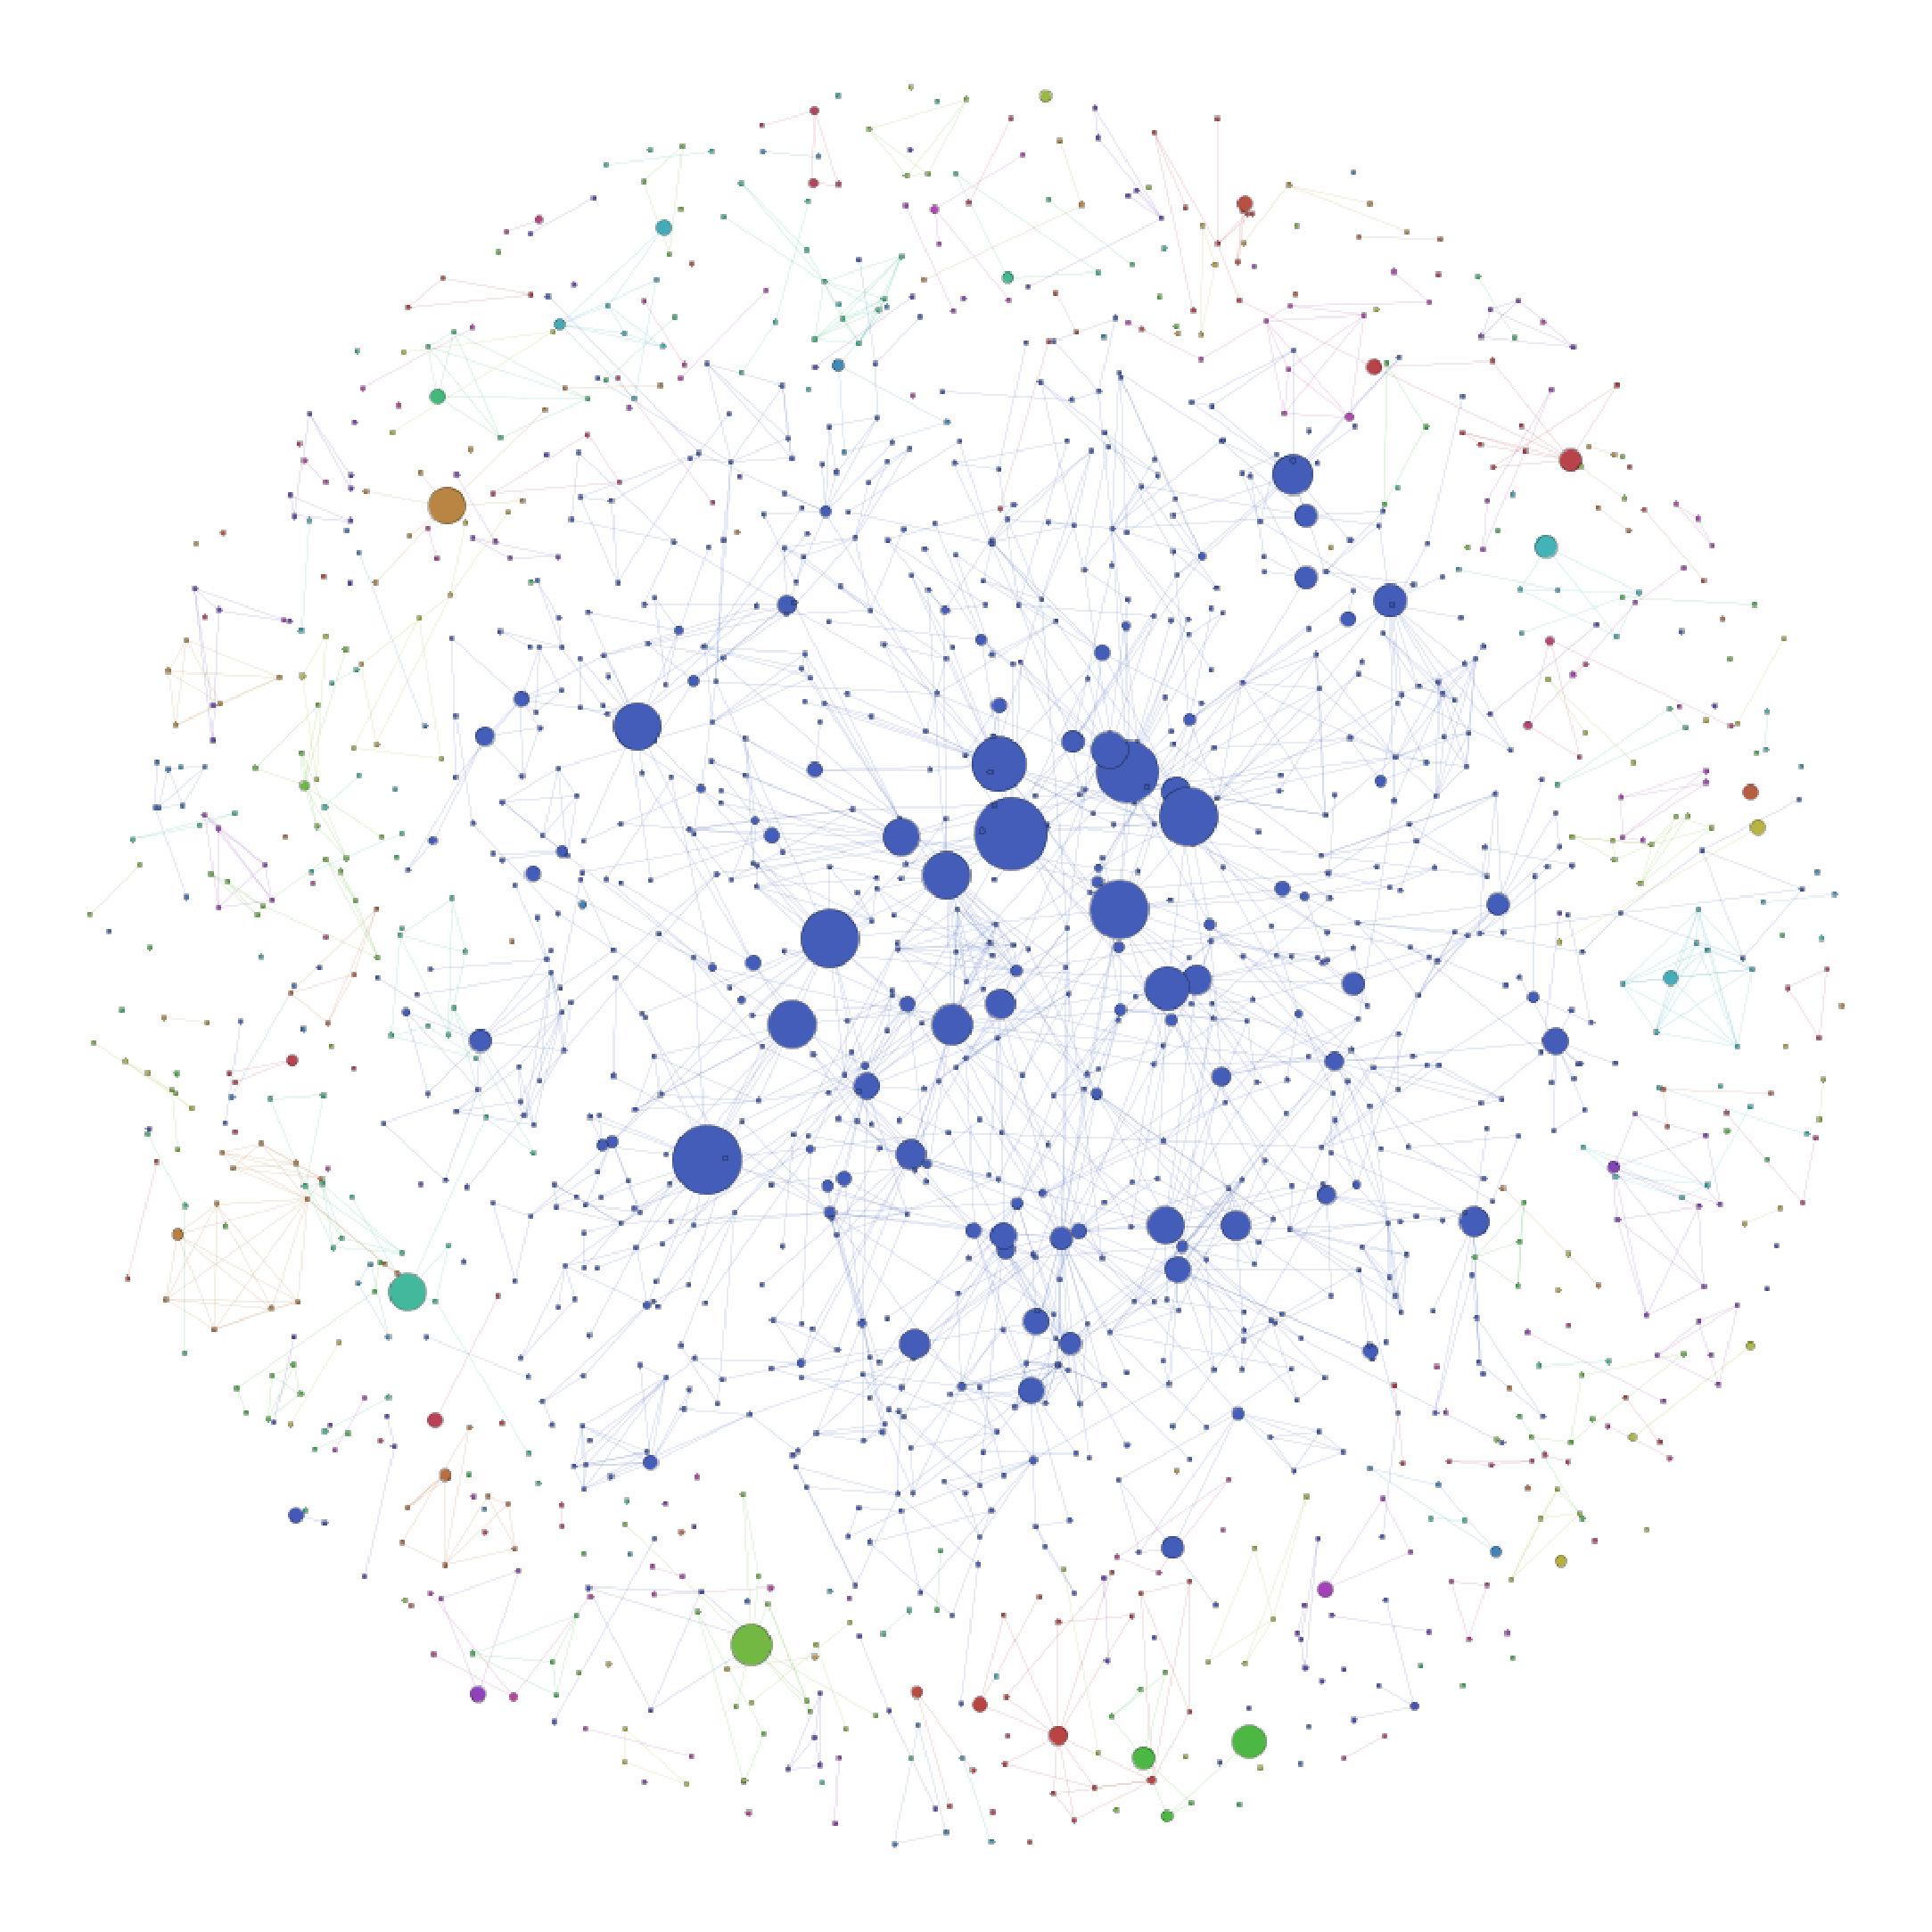
\includegraphics[scale=.21]{../graficos/network/popl.eps}
  }%
  \\
  \subfloat[SIGCOMM]{%
    \label{fig:rede_sigcomm_apendice}
    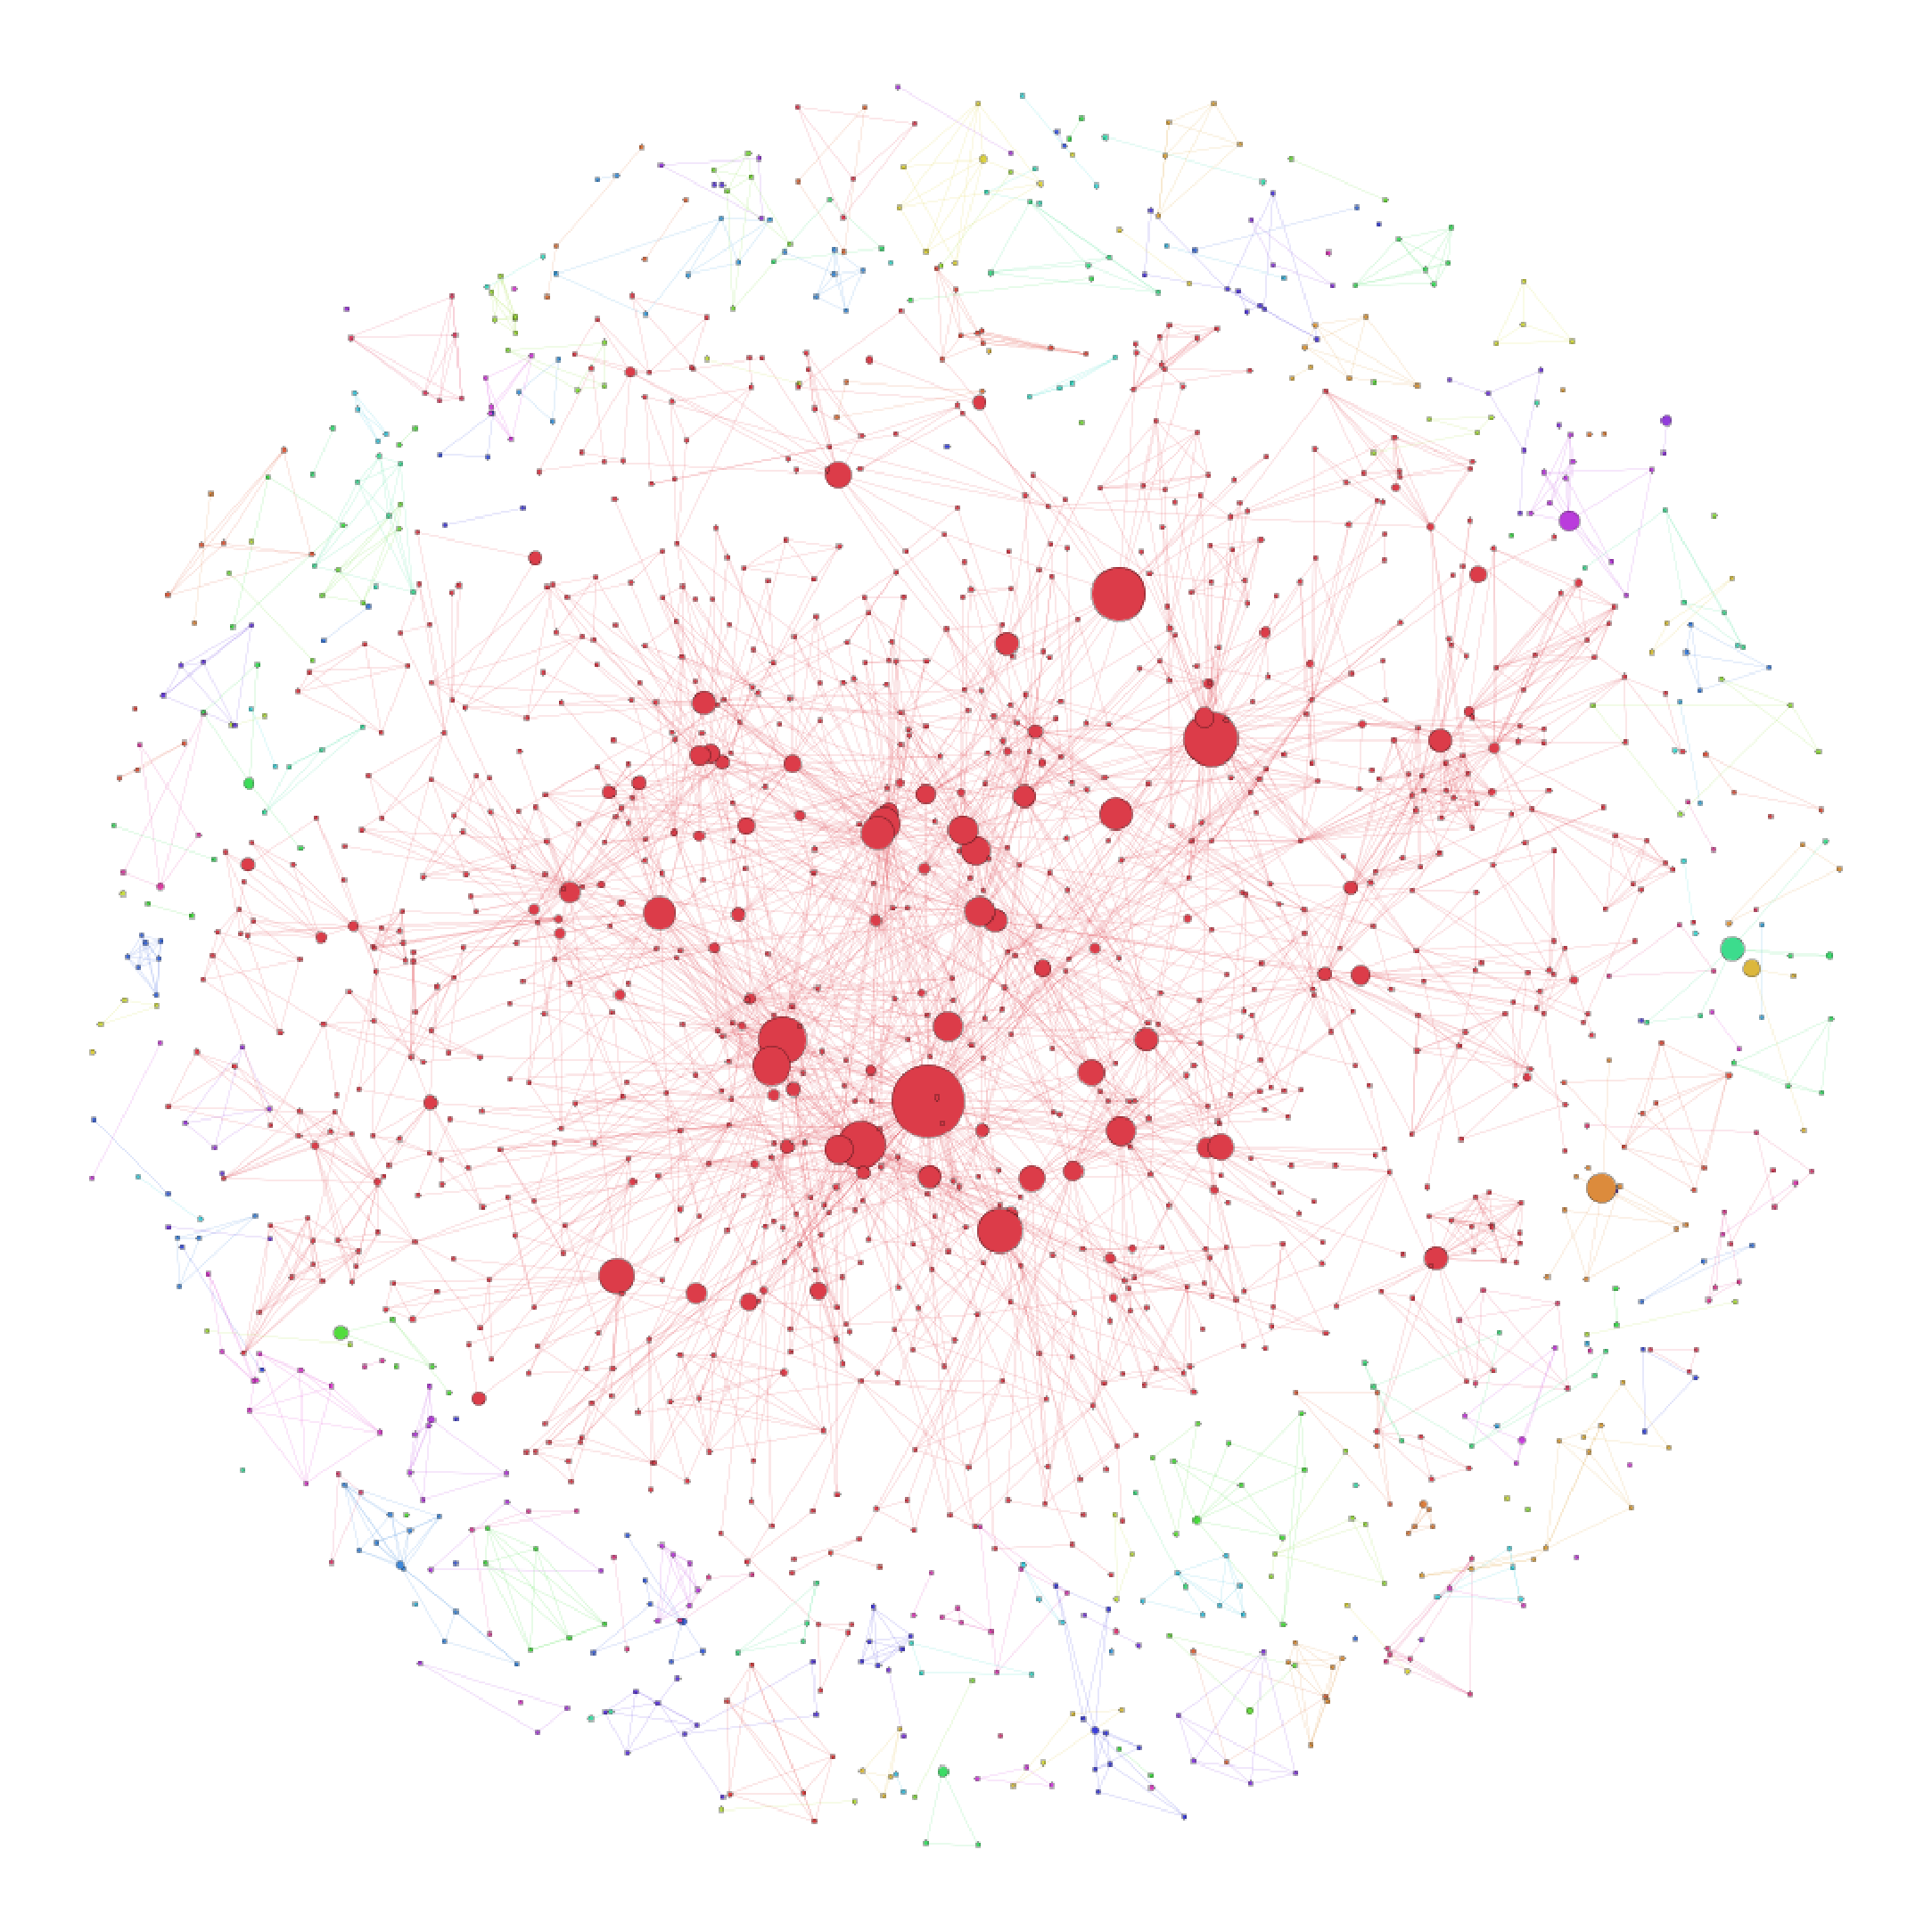
\includegraphics[scale=.21]{../graficos/network/sigcomm.eps}
  }%
  \subfloat[SIGCSE]{%
    \label{fig:rede_sigcse_apendice}
    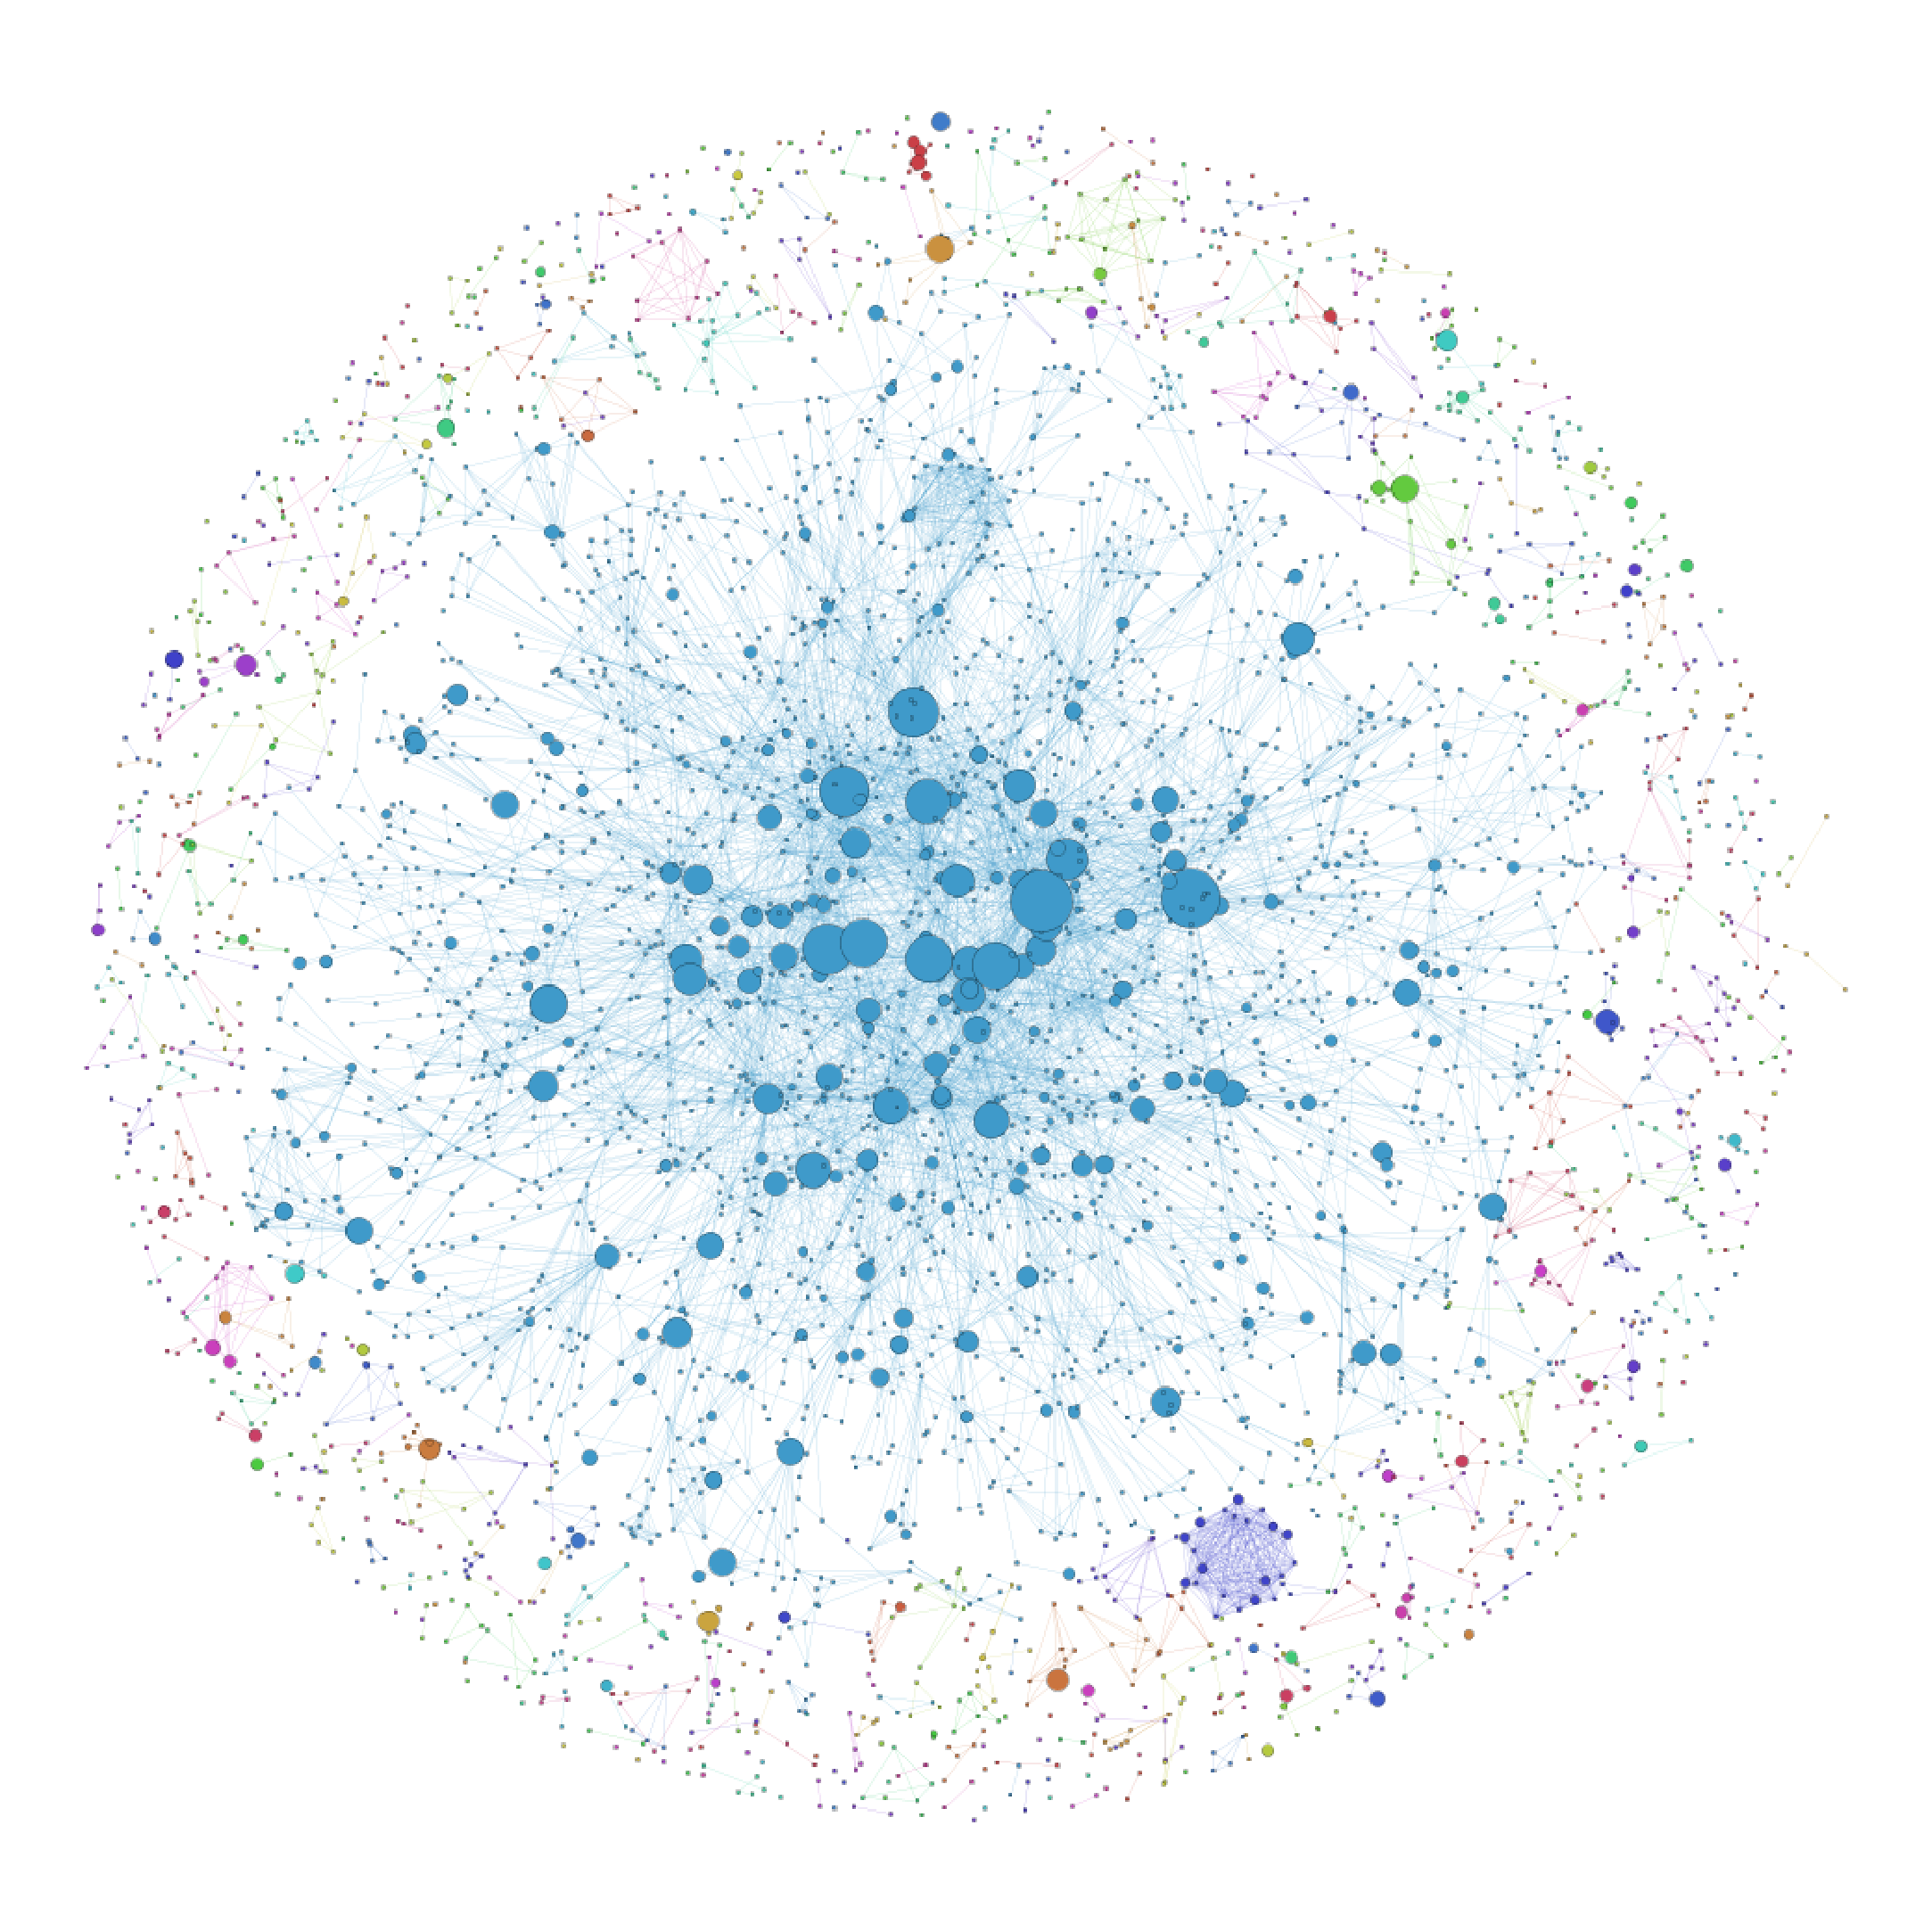
\includegraphics[scale=.21]{../graficos/network/sigcse.eps}
  }%
  \phantomcaption
  \end{center}
\end{figure}
\begin{figure}[!htb]
  \begin{center}
  \ContinuedFloat
  \subfloat[SIGDOC]{%
    \label{fig:rede_sigdoc_apendice}
    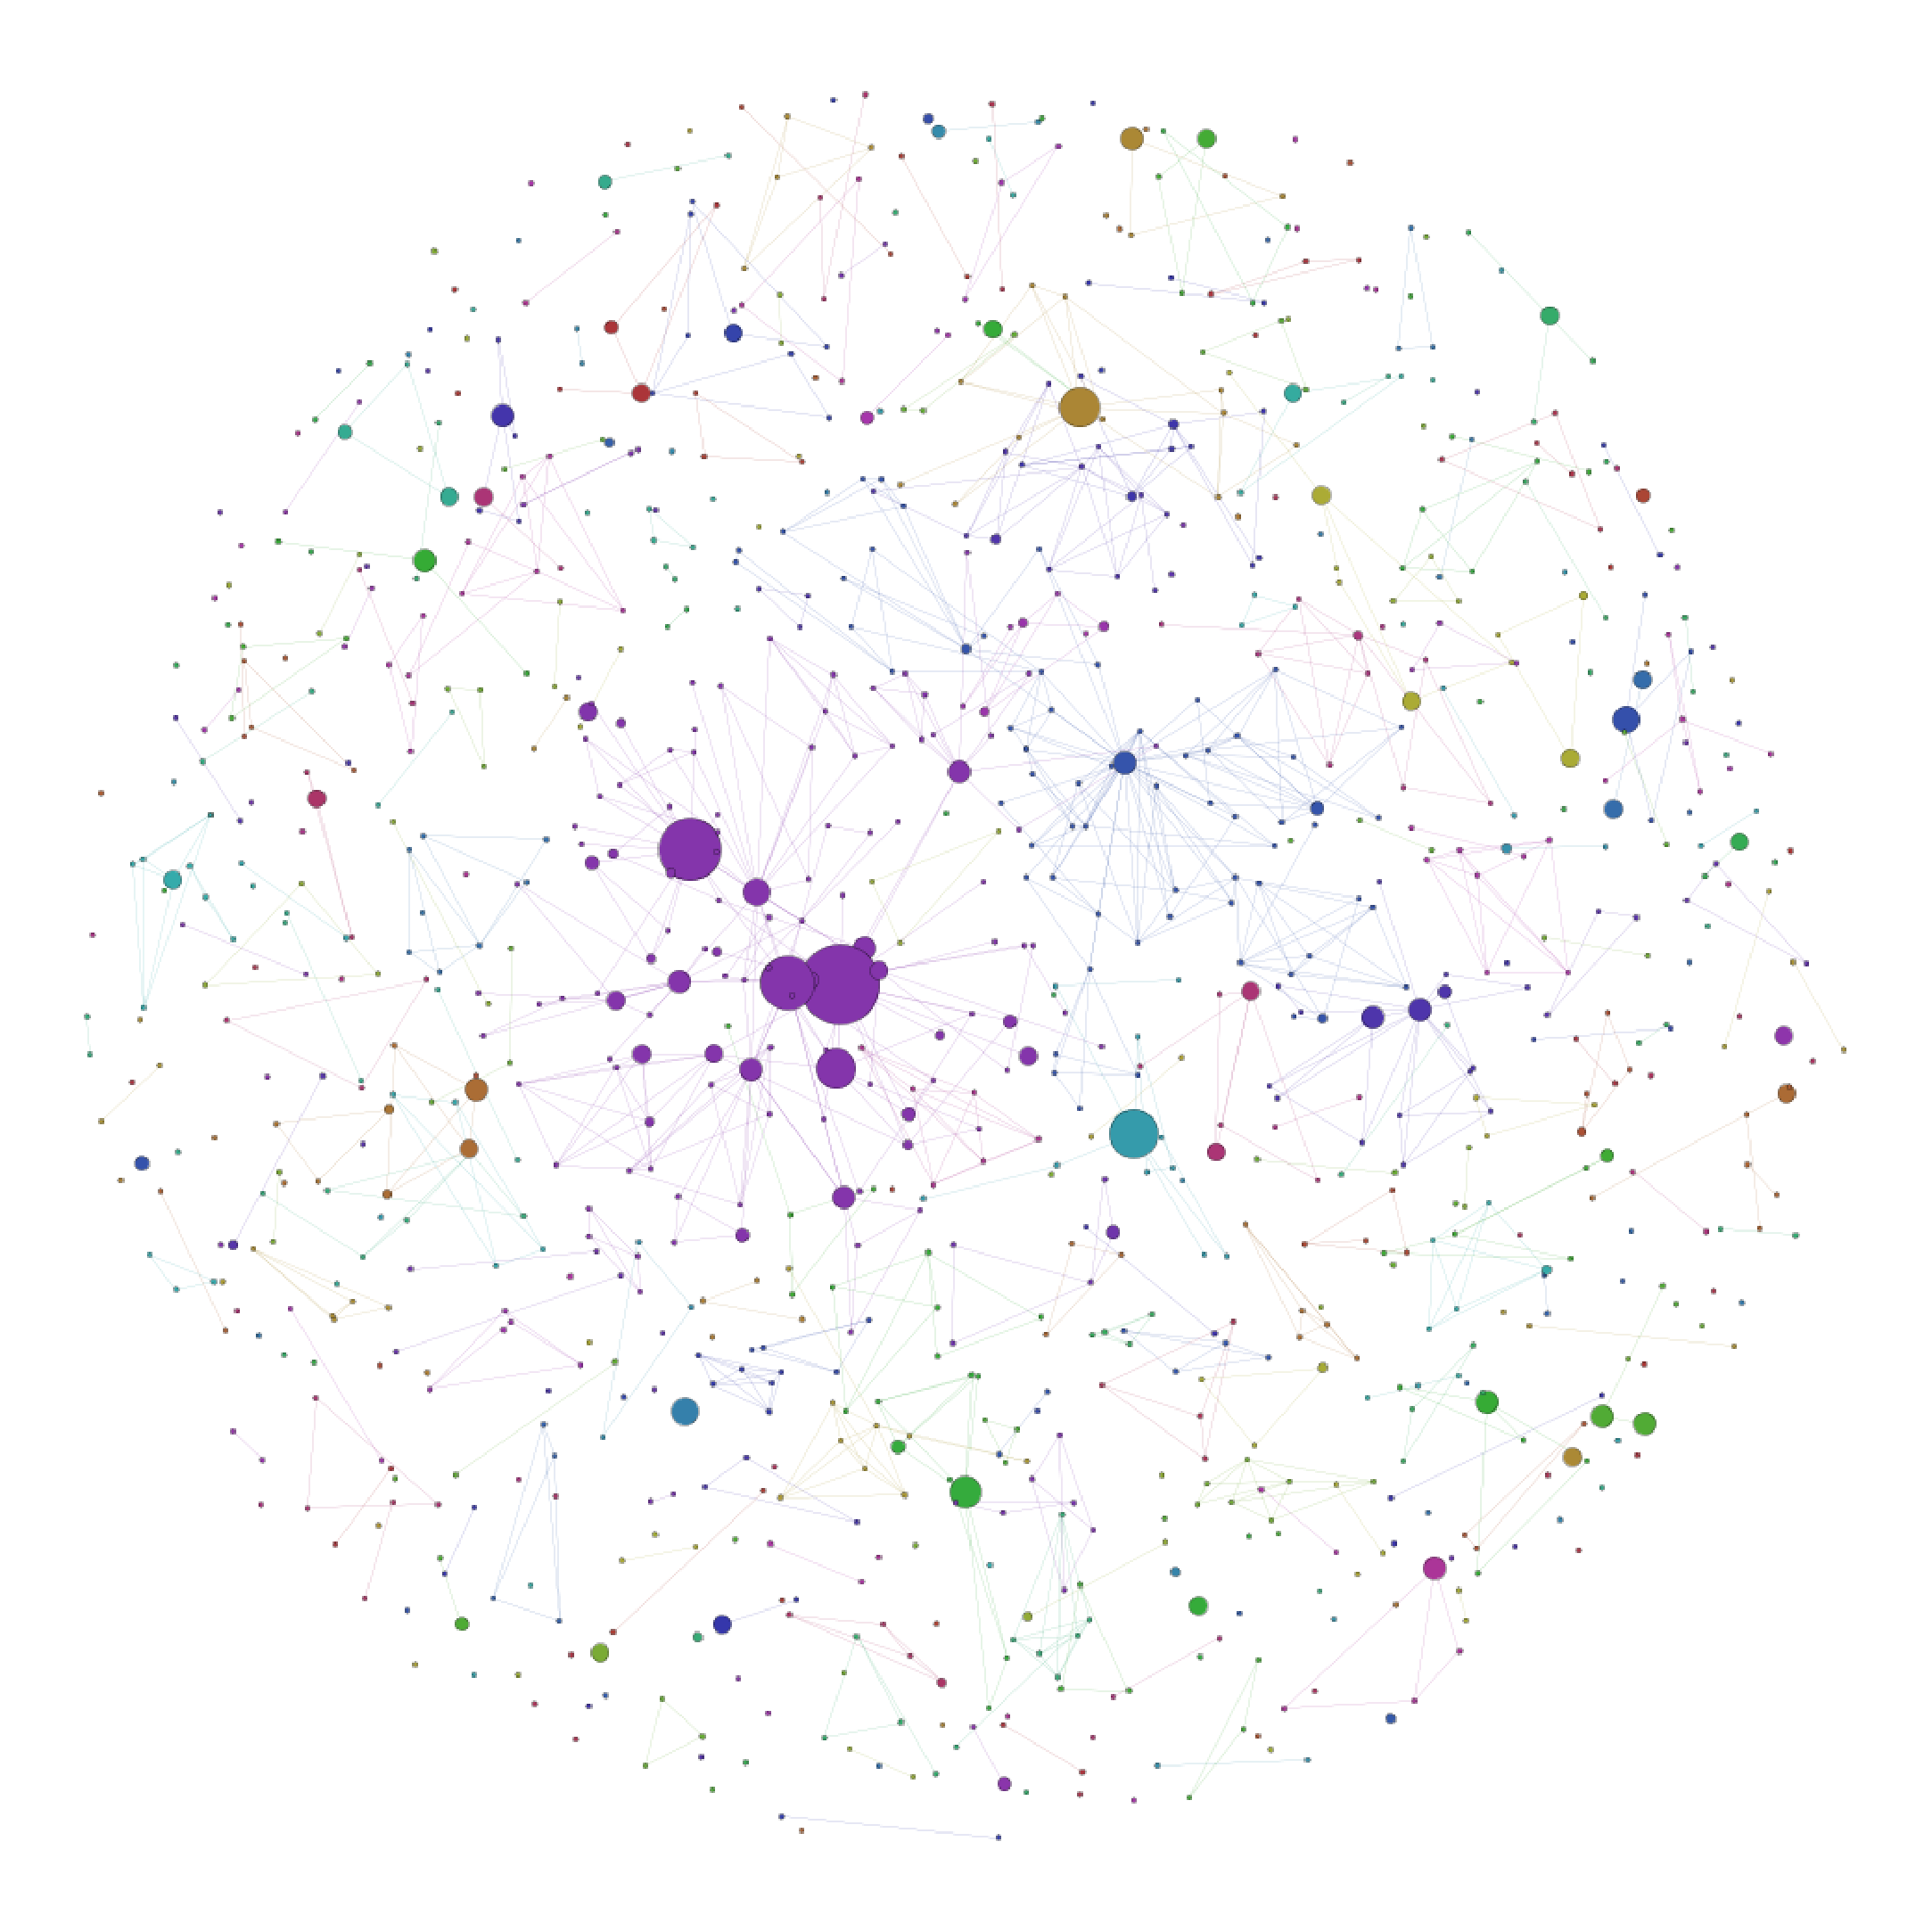
\includegraphics[scale=.21]{../graficos/network/sigdoc.eps}
  }%
  \subfloat[SIGGRAPH]{%
    \label{fig:rede_siggraph_apendice}
    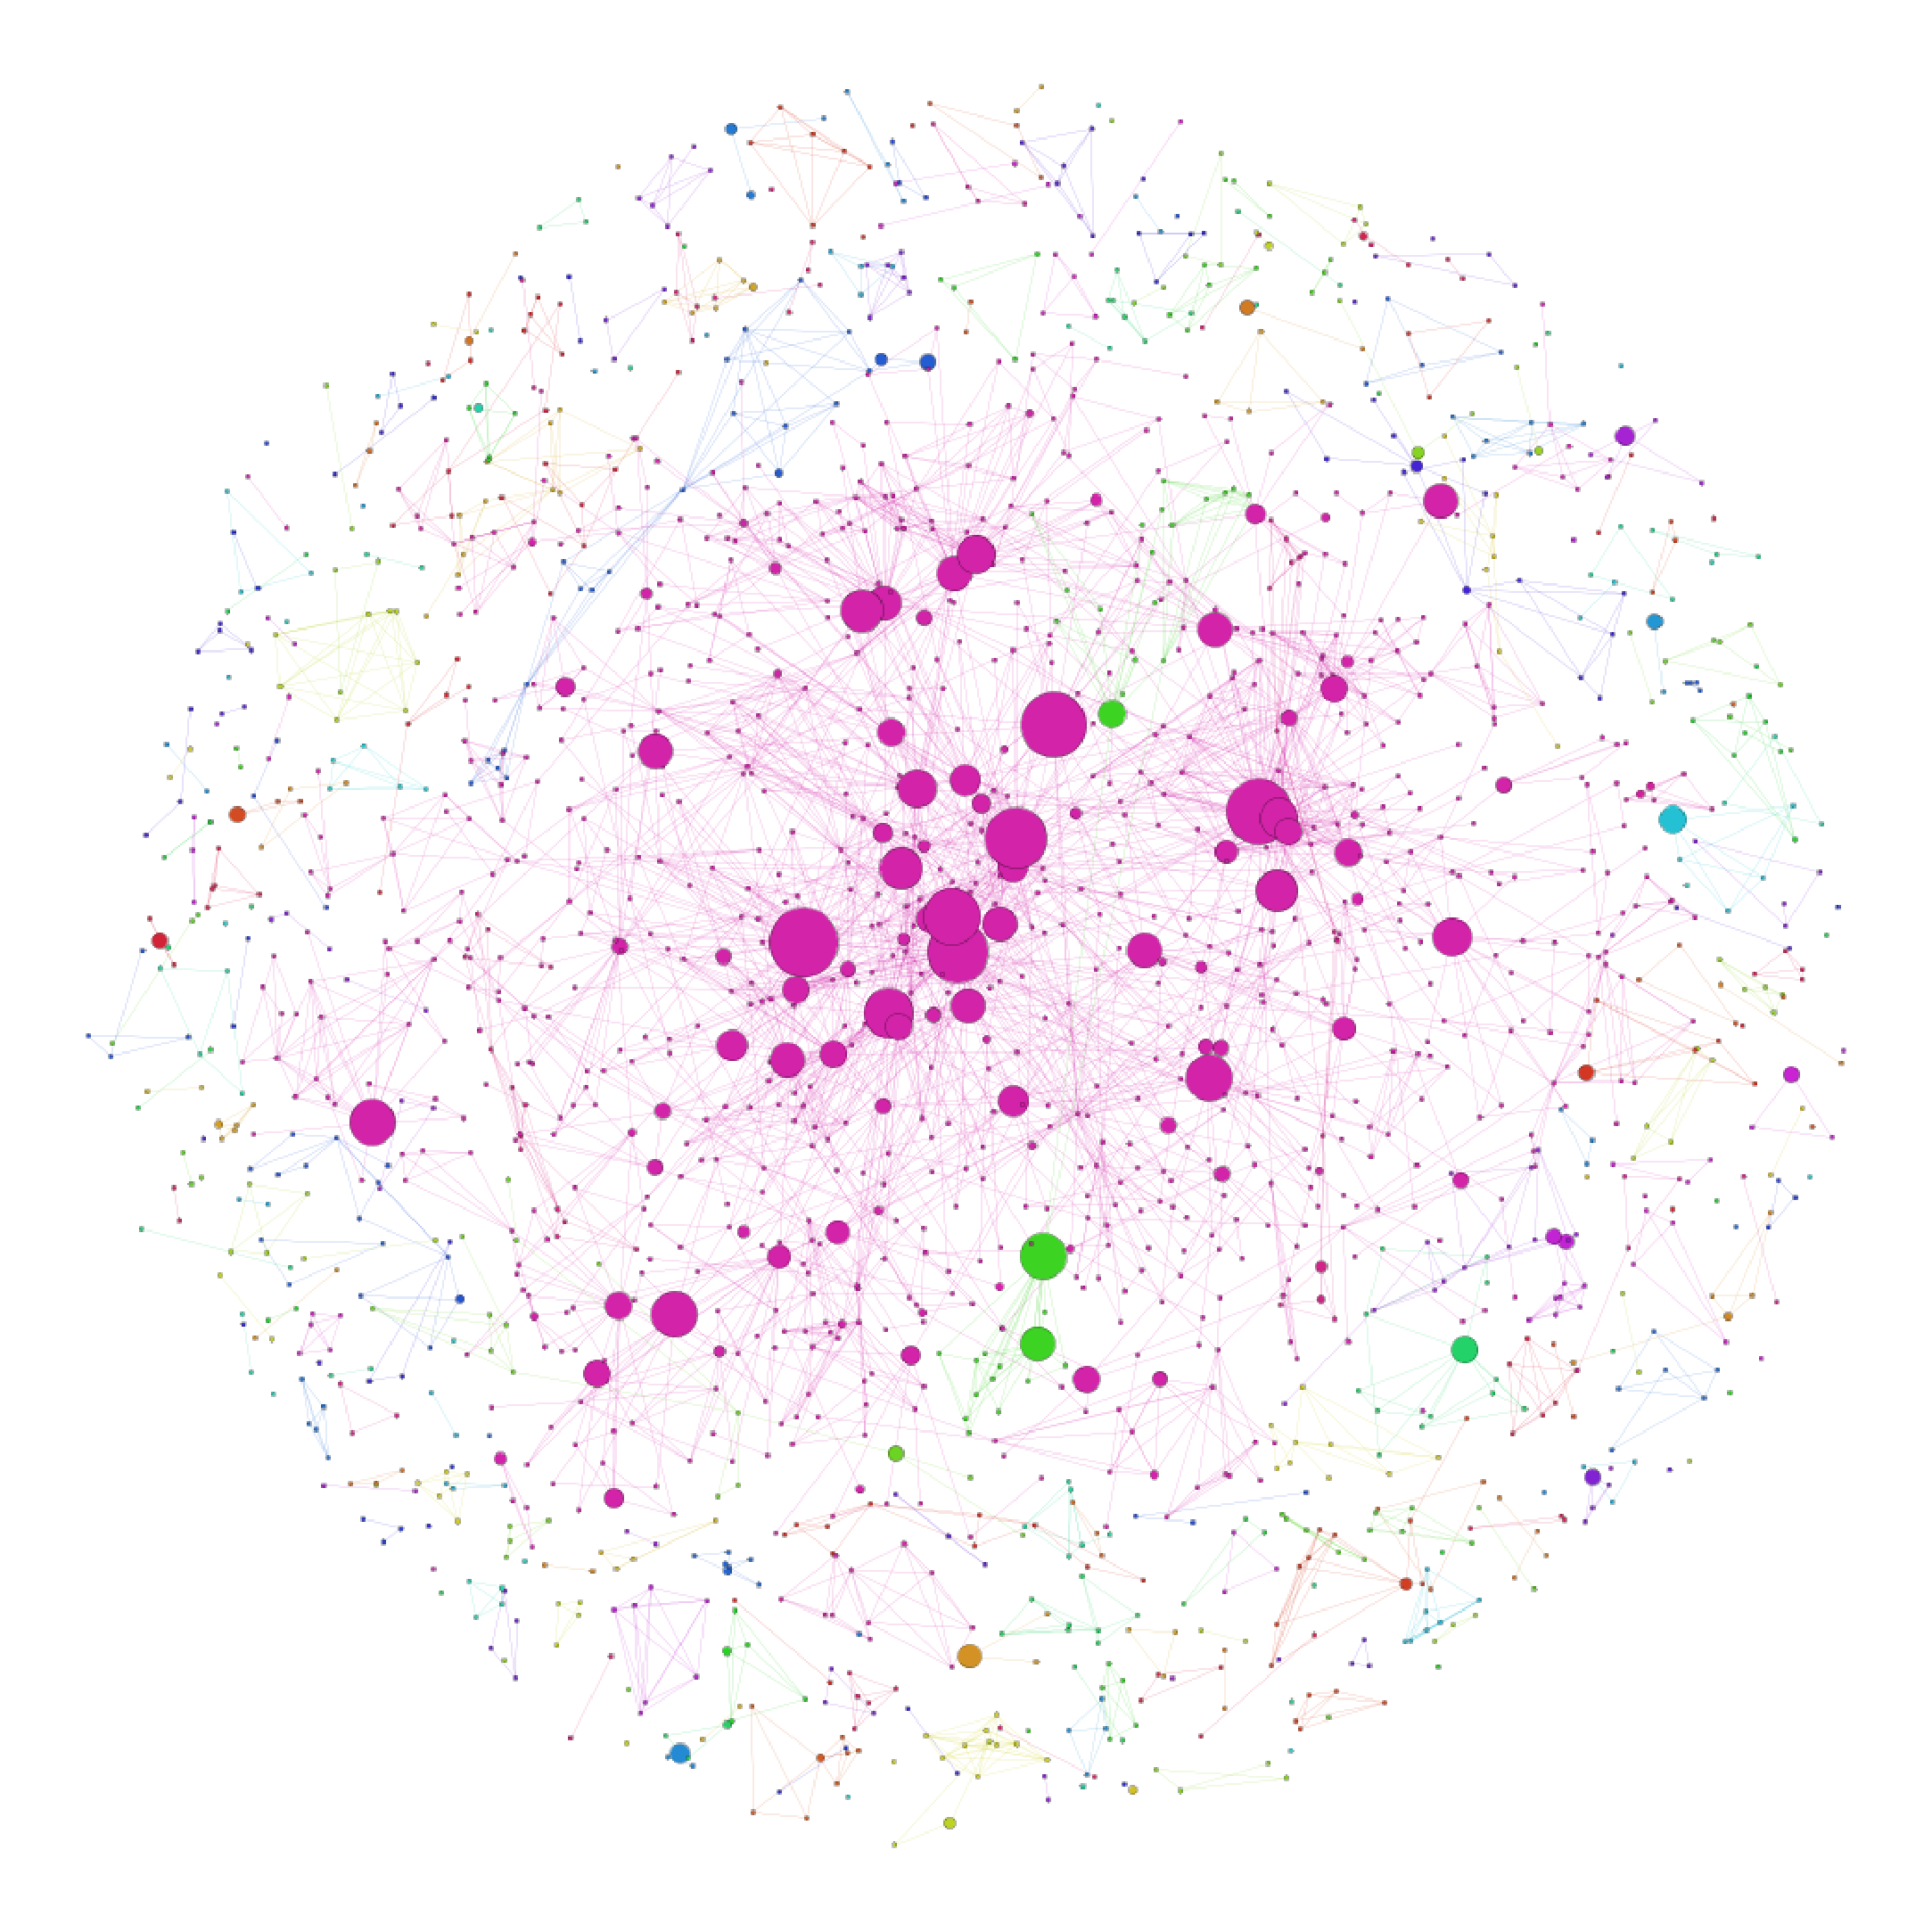
\includegraphics[scale=.21]{../graficos/network/siggraph.eps}
  }%
  \\
  \subfloat[SIGIR]{%
    \label{fig:rede_sigir_apendice}
    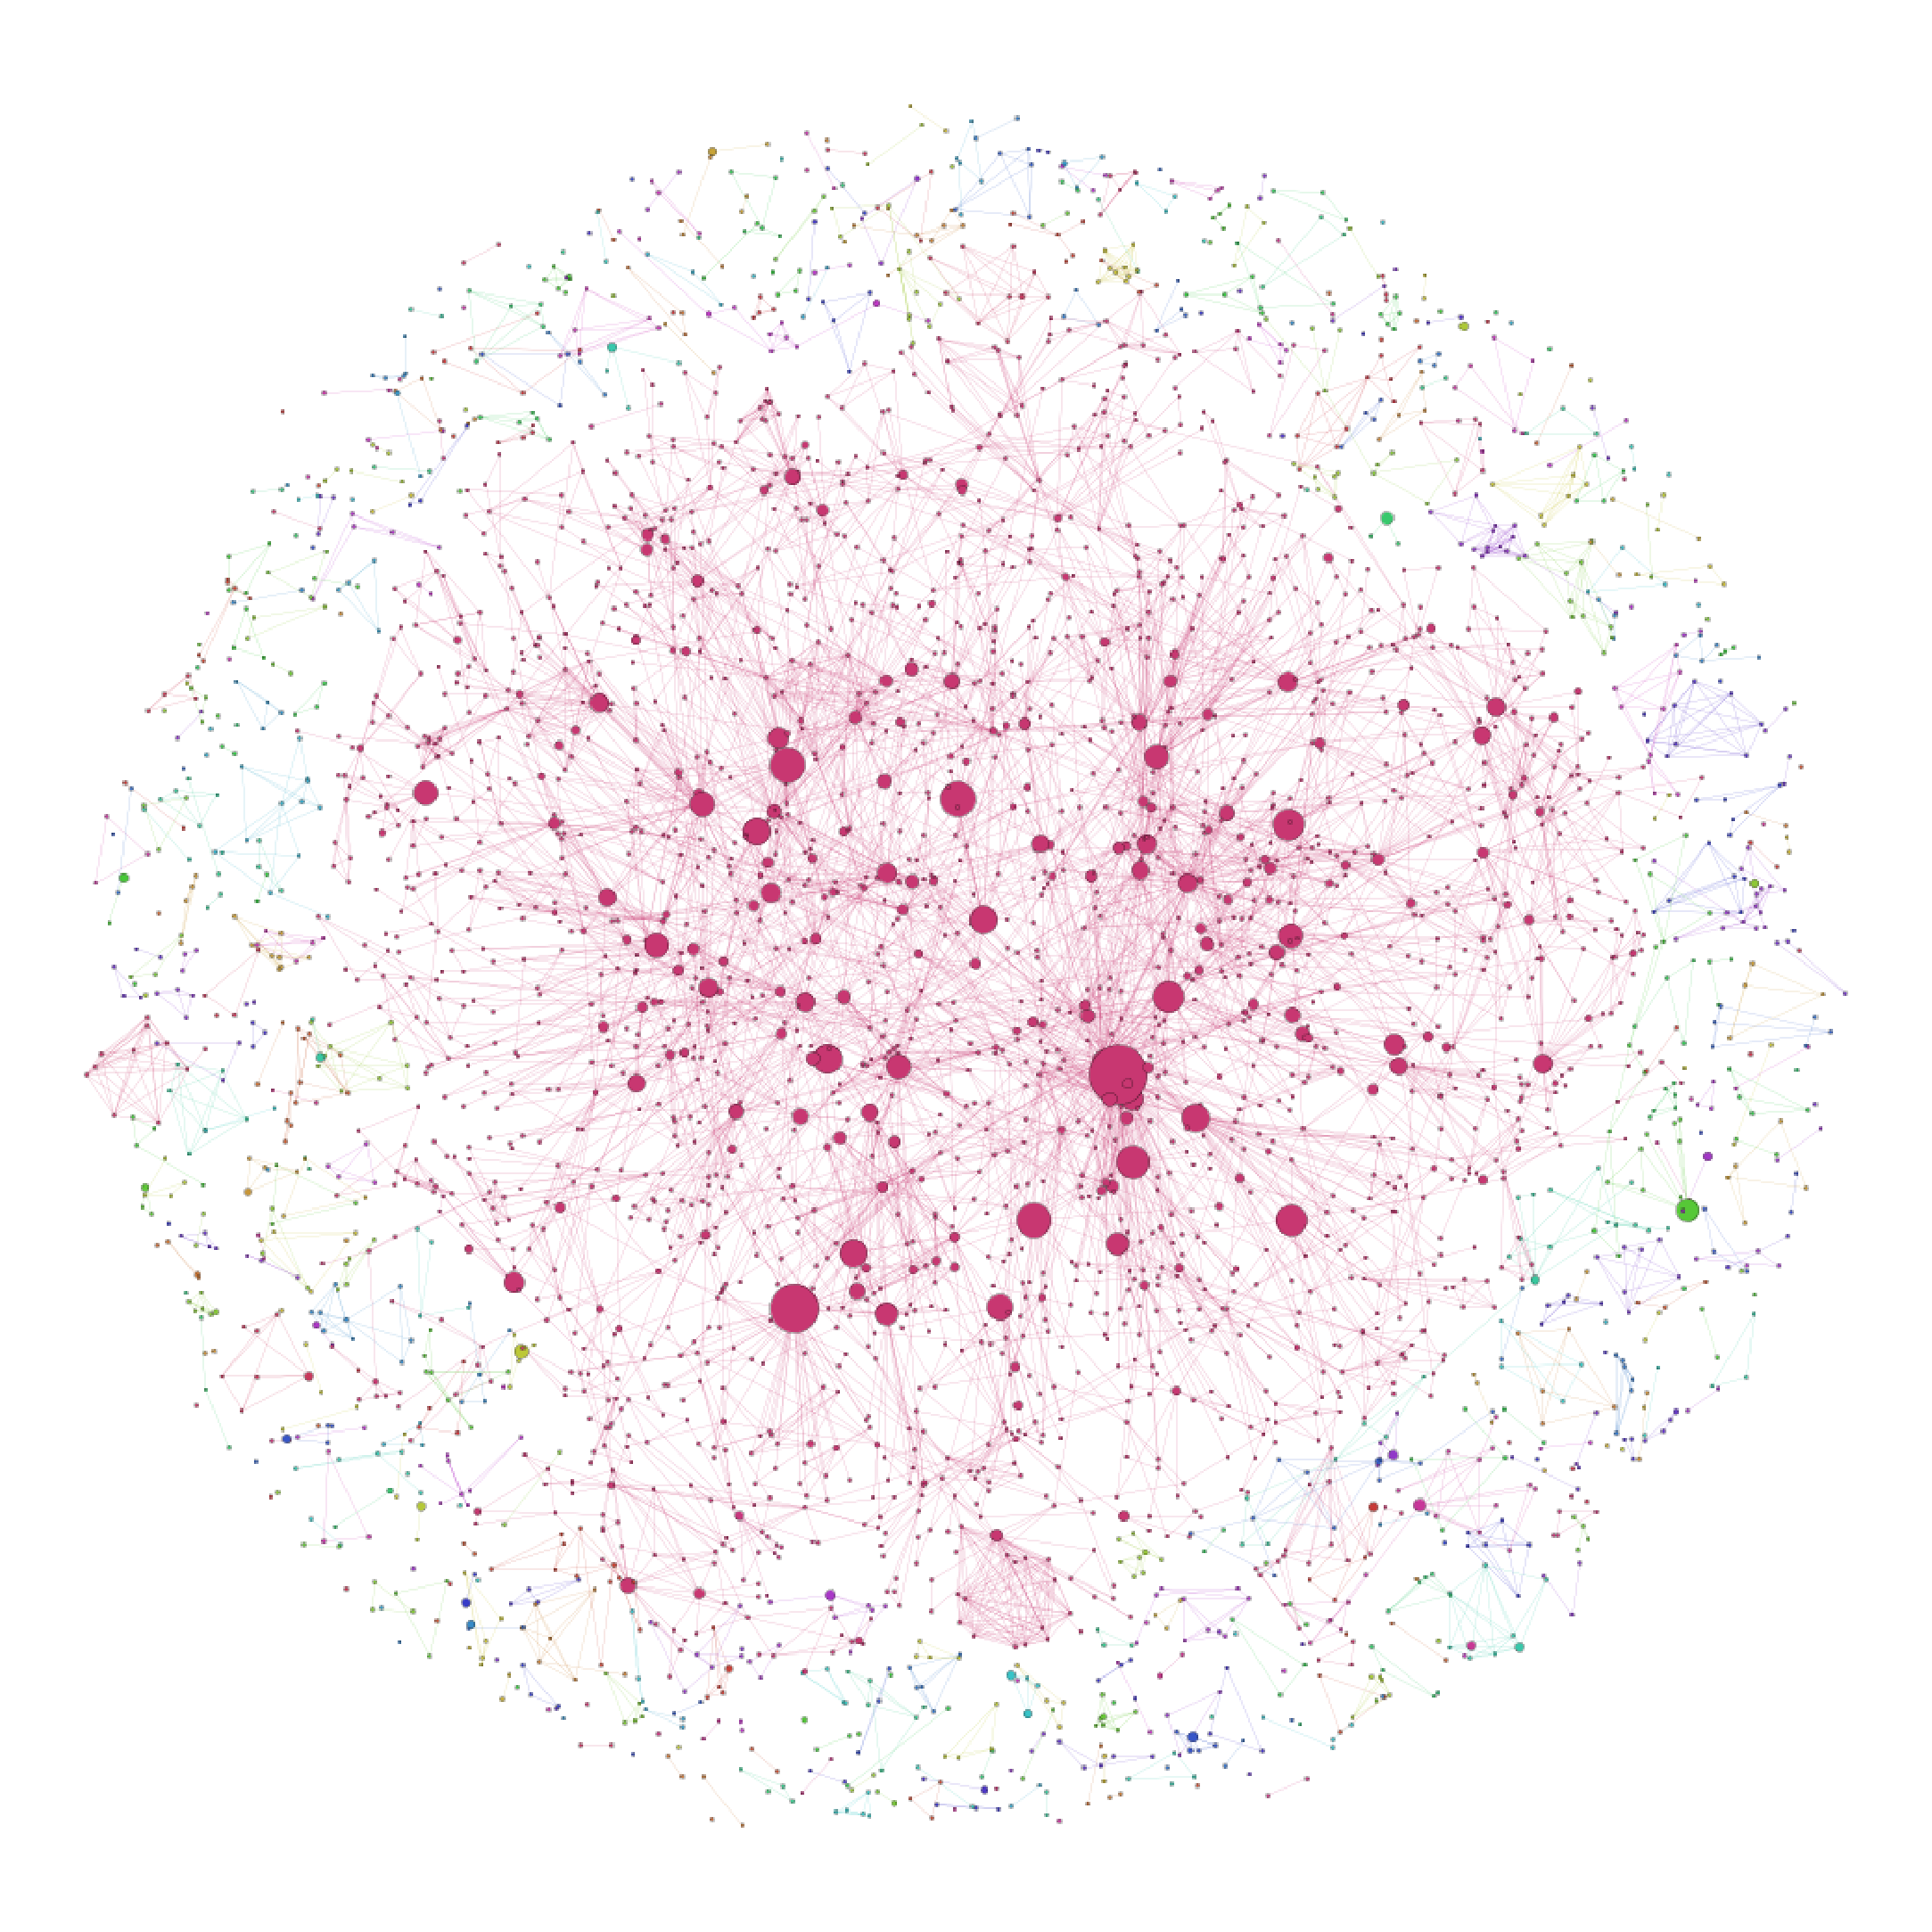
\includegraphics[scale=.21]{../graficos/network/sigir.eps}
  }%
  \subfloat[SIGMETRICS]{%
    \label{fig:rede_sigmetrics_apendice}
    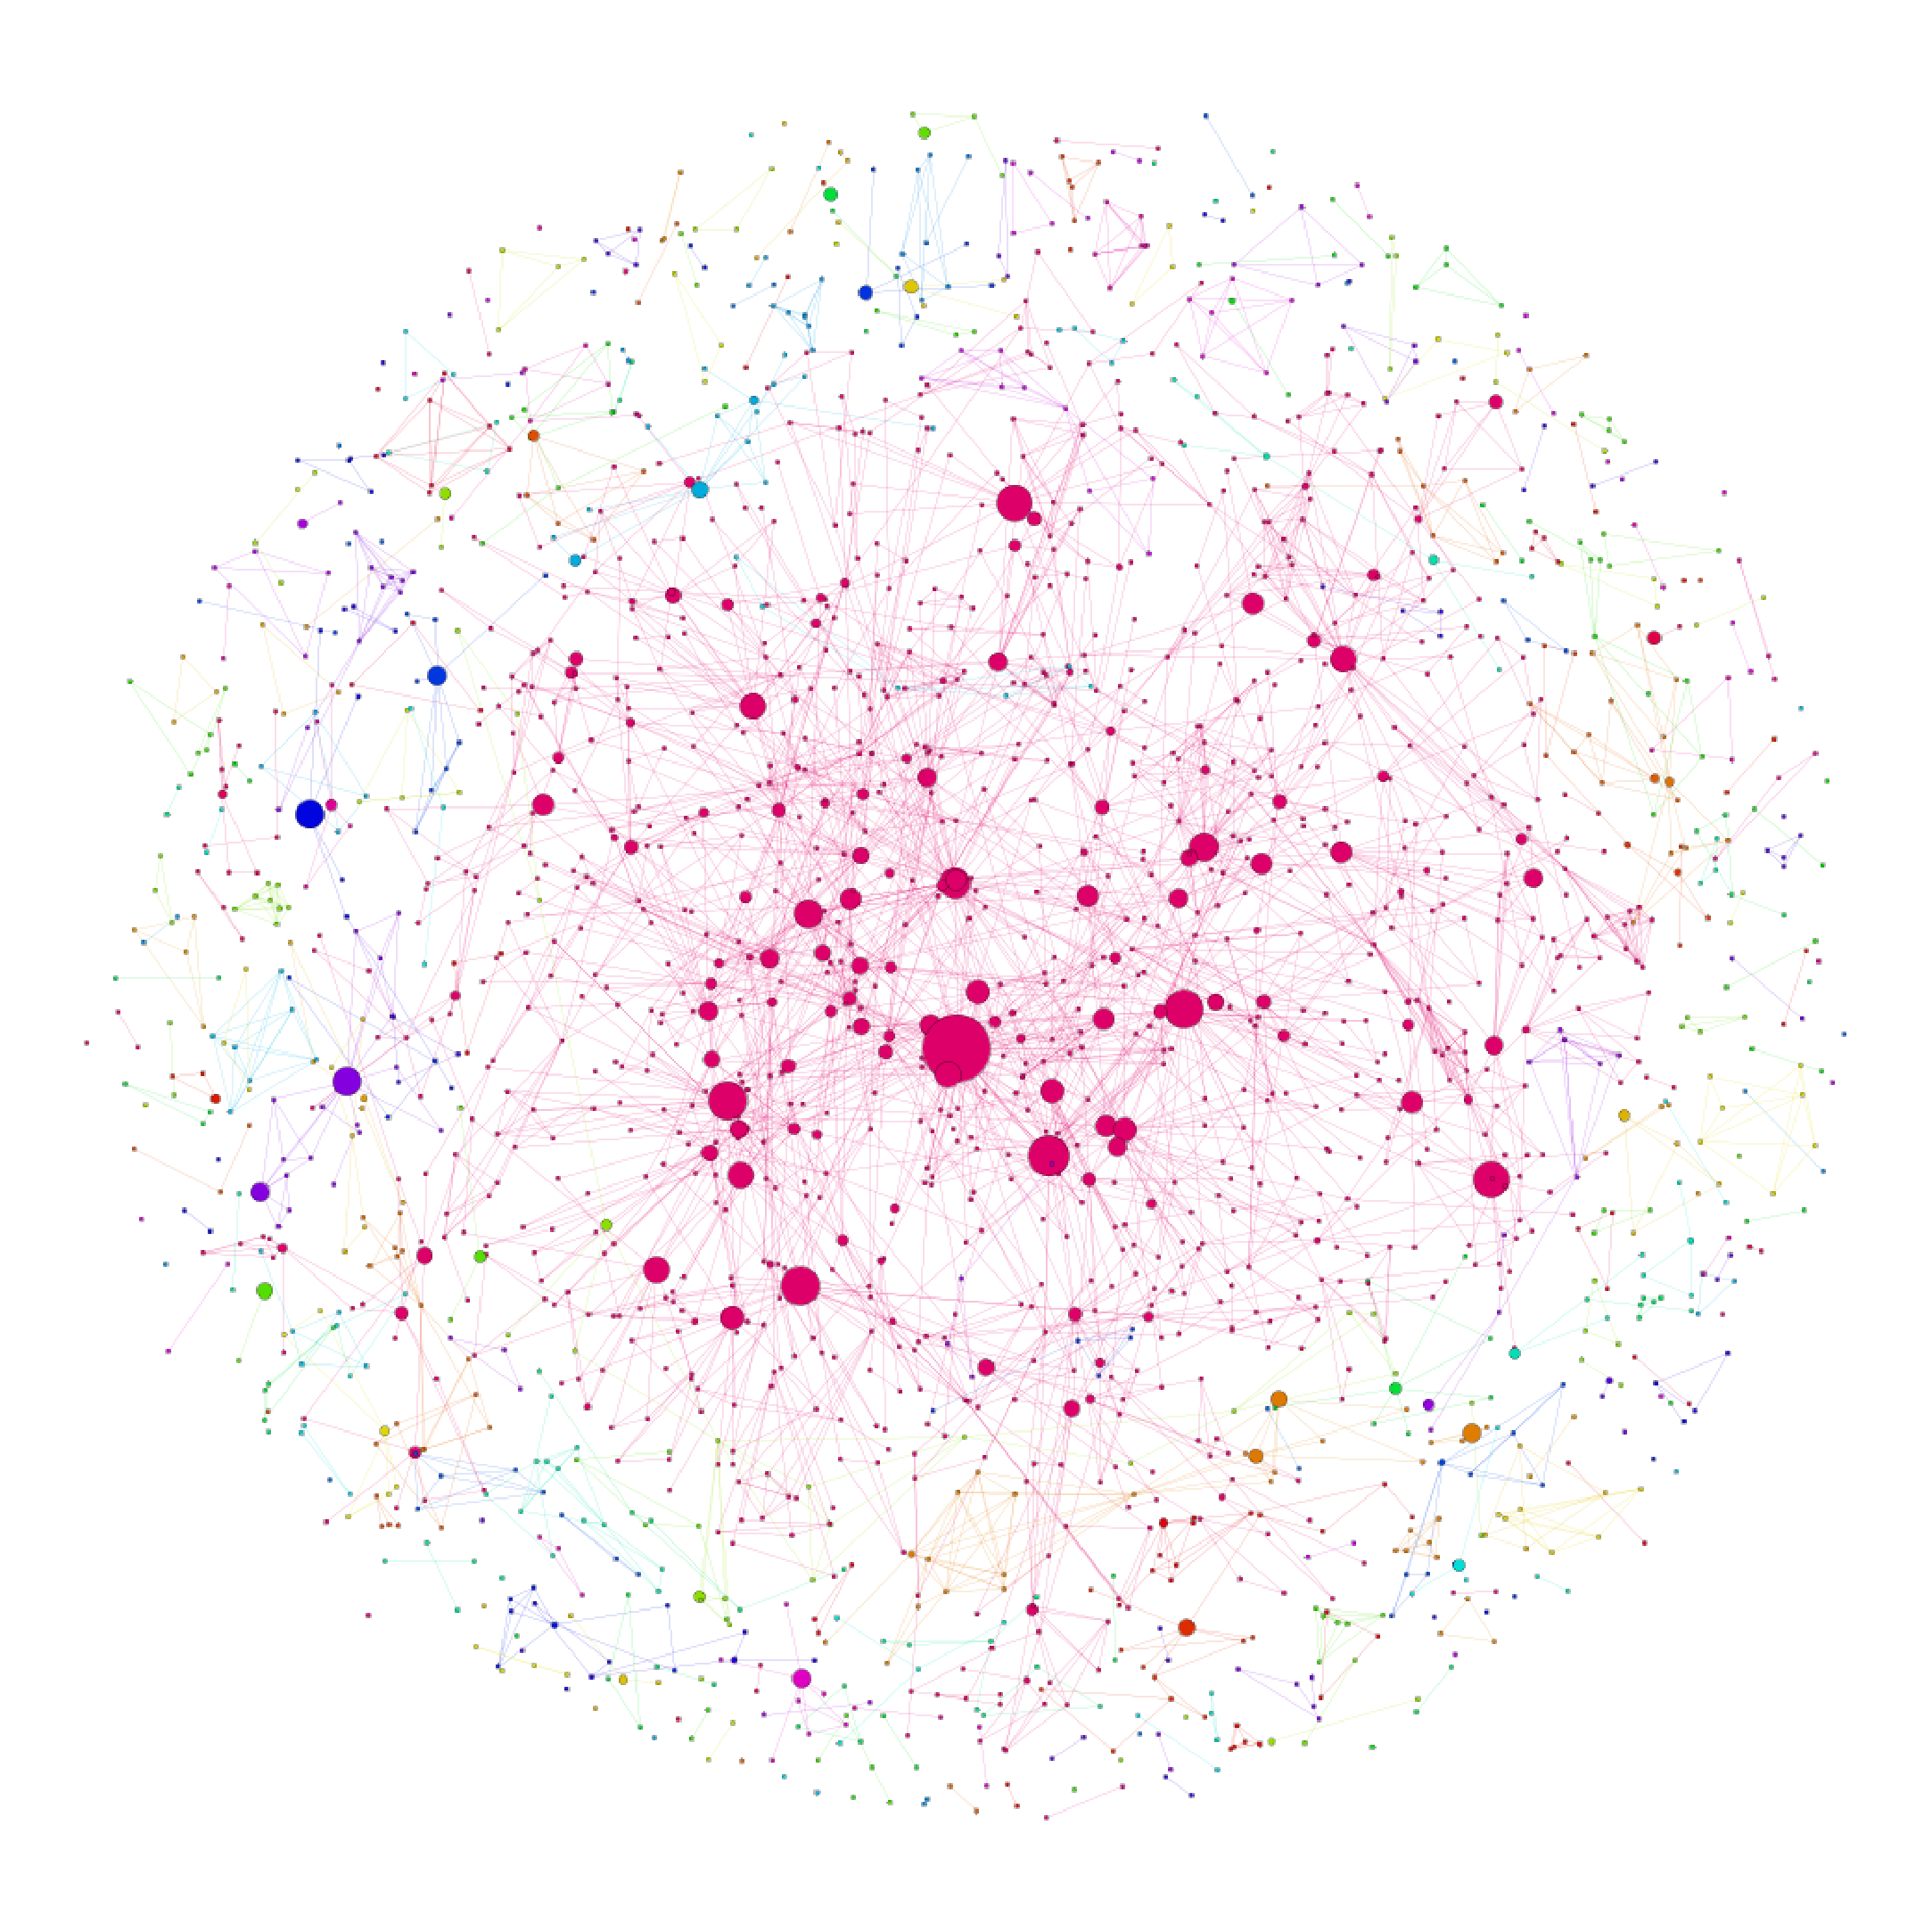
\includegraphics[scale=.21]{../graficos/network/sigmetrics.eps}
  }%
  \end{center}
  \caption{Instância final das comunidades científicas}
  \label{fig:redes_apendice}
\end{figure}